\lecture{类模板与STL编程}{lec:chap07}
\section[概念]{类模板的概念}\label{sec:chap07-sec01}
%%%%%%%%%%%%%%%%%%%%%%%%%%%%%% 继承与派生的概念 %%%%%%%%%%%%%%%%%%%%%%%%%%%%%%%%%%
% \begin{frame}[t, fragile]{类模板的概念}%
%   \begin{itemize}
%   \item 函数模板的回顾
%   \item 类模板的定义
%   \item 类模板的实例化
%   \item 带默认参数的类模板
%   \end{itemize}
% \end{frame}

\begin{frame}[t, fragile]{基本概念}{回顾:函数模板}%
  \begin{itemize}
  \item 函数模板(function templates or generic functions)\\
    \begin{center}
      \begin{minipage}[t]{0.6\linewidth}
        \begin{cppttnobg}
template <class |类型名|1, class |类型名|2, |$\cdots$|>
|返回类型| |函数名| (|形参表|)
{
  |$\cdots$|
}
        \end{cppttnobg}
      \end{minipage}
    \end{center} 
  \end{itemize}
\end{frame}

\begin{frame}[t, fragile]{基本概念}{回顾:函数模板}%
  \begin{itemize}
  \item 利用函数模板进行求和运算
  \end{itemize}
  \begin{center}
    \begin{tikzpicture}[font=\tiny, show background grid]
      \tikzset{ coord/.style={coordinate} }
      
      \umlnote[text width=0.65\textwidth](code1) at (0, 0)
      {
        \cppfilenobg{codes/chap07/01-funtemplate.cpp}
      };      

      \path let \p1=(code1) in
      coordinate (org) at (\x1, \y1)
      coordinate (ovBL1) at ($(org) + (-4.24, 0.375)$)
      coordinate (ovUR1) at ($(ovBL1) + (3.0, 0.26)$)
      ;

      \path let \p1=(code1) in
      coordinate (org) at (\x1, \y1)
      coordinate (ovBL2) at ($(org) + (-2.76, -1.99)$)
      coordinate (ovUR2) at ($(ovBL2) + (0.95, 0.26)$)
      ;

      \draw[red,thick,fill=green!35, fill opacity=0.3](ovBL1) rectangle
      (ovUR1);
      \draw[blue,thick,fill=red!35, fill opacity=0.3](ovBL2) rectangle
      (ovUR2);
      
    \end{tikzpicture}
  \end{center}
\end{frame}

\begin{frame}[t, fragile]{基本概念}{类模板的定义}%
  \begin{spacing}{1.5}
  \begin{itemize}
  \item 类模板(class templates or generic classes)定义\\
    \begin{center}
      \begin{minipage}[t]{0.65\linewidth}
        \begin{cppttnobg}
        |或|typename |$\cdots$|,   |或|typename |$\cdots$|
template <class |参数化类型|1, class |参数化类型|2, |$\cdots$|,
          |普通类型|1, |普通类型|2, |$\cdots$|>
class |类名|
{
  |成员名|;
}
        \end{cppttnobg}
      \end{minipage}
    \end{center} 
  \item 关于\cppinline{class}和\cppinline{typename},请参阅:\\[2ex]
    {\tiny
      \url{http://dev.yesky.com/13/2221013.shtml}\\
      \url{http://blogs.msdn.com/b/slippman/archive/2004/08/11/212768.aspx}
    }
  \end{itemize}
  \end{spacing}
\end{frame}

\begin{frame}[t, fragile]{基本概念}{类模板的定义}%
  \begin{itemize}
  \item 安全数组类模板的定义
  \end{itemize}
  \begin{center}
    \begin{tikzpicture}[font=\tiny, show background grid]
      \tikzset{ coord/.style={coordinate} }
      
      \umlnote[text width=0.7\textwidth](code1) at (0, 0)
      {
        \cppfilenobg{codes/chap07/02-classtemplate.cpp}
      };      

      \path let \p1=(code1) in
      coordinate (org) at (\x1, \y1)
      coordinate (ovBL1) at ($(org) + (-3.6, 1.92)$)
      coordinate (ovUR1) at ($(ovBL1) + (0.95, 0.26)$)
      coordinate (ovBR1) at ($(ovBL1) + (1.0, 0.0)$)
      coordinate (ovMR1) at ($(ovUR1)!0.5!(ovBR1)$)
      coordinate (ovMB1) at ($(ovBL1)!0.5!(ovBR1)$)
      ;

      \node[fill=blue!25, draw, yshift = -0.7cm, right=2 of ovMR1]
      (note1) {参数化类型};

      \draw[red,thick,fill=green!35, fill opacity=0.3](ovBL1) rectangle
      (ovUR1);
      
      \draw[-{Stealth[scale=1.0]}, red, thick] (note1.west) to[out =
      180, in = -90] (ovMB1);      
    \end{tikzpicture}
  \end{center}
\end{frame}

\begin{frame}[t, fragile]{基本概念}{类模板的定义}%
  \begin{itemize}
  \item 安全数组类模板的定义
  \end{itemize}
  \begin{center}
    \begin{tikzpicture}[font=\tiny, show background grid]
      \tikzset{ coord/.style={coordinate} }
      
      \umlnote[text width=0.7\textwidth](code1) at (0, 0)
      {
        \cppfilenobg{codes/chap07/02-classtemplate.cpp}
      };      

      \path let \p1=(code1) in
      coordinate (org) at (\x1, \y1)
      coordinate (ovBL1) at ($(org) + (-2.72, 1.92)$)
      coordinate (ovUR1) at ($(ovBL1) + (0.95, 0.26)$)
      coordinate (ovBR1) at ($(ovBL1) + (1.0, 0.0)$)
      coordinate (ovMR1) at ($(ovUR1)!0.5!(ovBR1)$)
      coordinate (ovMB1) at ($(ovBL1)!0.5!(ovBR1)$)
      ;

      \node[fill=blue!25, draw, yshift = -0.7cm, right=2 of ovMR1]
      (note1) {普通类型};

      \draw[red,thick,fill=green!35, fill opacity=0.3](ovBL1) rectangle
      (ovUR1);
      
      \draw[-{Stealth[scale=1.0]}, red, thick] (note1.west) to[out =
      180, in = -90] (ovMB1);      
    \end{tikzpicture}
  \end{center}
\end{frame}

\begin{frame}[ t, fragile]{基本概念}{类模板的定义}%
  \begin{itemize}
  \item 类模板中的成员函数→函数模板
  \end{itemize}
  \begin{center}
    \begin{tikzpicture}[font=\tiny, show background grid]
      \tikzset{ coord/.style={coordinate} }
      
      \umlnote[text width=0.7\textwidth](code1) at (0, 0)
      {
        \cppfilenobg{codes/chap07/02-classtemplate.cpp}
      };      

      \path let \p1=(code1) in
      coordinate (org) at (\x1, \y1)
      coordinate (ovBL1) at ($(org) + (-4.32, -0.45)$)
      coordinate (ovUR1) at ($(ovBL1) + (2.10, 0.30)$)
      coordinate (ovBR1) at ($(ovBL1) + (2.3, 0.0)$)
      coordinate (ovMR1) at ($(ovUR1)!0.5!(ovBR1)$)
      coordinate (ovMB1) at ($(ovBL1)!0.5!(ovBR1)$)
      ;

      \node[fill=blue!25, draw, yshift = -0.5cm, right=2 of ovMR1]
      (note1) {函数模板};

      \draw[red,thick,fill=green!35, fill opacity=0.3](ovBL1) rectangle
      (ovUR1);
      
      \draw[-{Stealth[scale=1.0]}, red, thick] (note1.west) to[out =
      180, in = 0] (ovMR1);      
    \end{tikzpicture}
  \end{center}
\end{frame}

\begin{frame}[t, fragile]{基本概念}{类模板的定义}%
  \begin{itemize}
  \item 类外定义类模板成员函数
  \end{itemize}
  \begin{center}
    \begin{tikzpicture}[font=\tiny, show background grid]
      \tikzset{ coord/.style={coordinate} }
      
      \umlnote[text width=0.55\textwidth](code1) at (0, 0)
      {
        \cppfilenobg{codes/chap07/03-operatortemplate.cpp}
      };

      \umlnote[text width=0.35\textwidth, yshift=-2.5cm, right=-2.2 of code1](code2)
      {
        \cppfilenobg{codes/chap07/04-operatortemplate.cpp}
      };

      \path let \p1=(code1) in
      coordinate (org) at (\x1, \y1)
      coordinate (ovBL1) at ($(org) + (-3.60, 0.99)$)
      coordinate (ovUR1) at ($(ovBL1) + (2.90, 0.26)$)
      coordinate (ovBR1) at ($(ovBL1) + (2.90, 0.0)$)
      coordinate (ovMR1) at ($(ovUR1)!0.5!(ovBR1)$)
      coordinate (ovMB1) at ($(ovBL1)!0.5!(ovBR1)$)
      ;

      \path let \p1=(code2) in
      coordinate (org) at (\x1, \y1)
      coordinate (ovBL2) at ($(org) + (-2.30, 0.80)$)
      coordinate (ovUR2) at ($(ovBL2) + (2.90, 0.26)$)
      coordinate (ovBR2) at ($(ovBL2) + (2.90, 0.0)$)
      coordinate (ovUL2) at ($(ovBL2) + (0.0, 0.26)$)
      coordinate (ovMR2) at ($(ovUR2)!0.5!(ovBR2)$)
      coordinate (ovMB2) at ($(ovBL2)!0.5!(ovBR2)$)
      coordinate (ovMA2) at ($(ovUL2)!0.5!(ovUR2)$) 
      ;

      \path let \p1=(code2) in
      coordinate (org) at (\x1, \y1)
      coordinate (ovBL3) at ($(org) + (-2.25, 0.55)$)
      coordinate (ovUR3) at ($(ovBL3) + (2.30, 0.26)$)
      coordinate (ovBR3) at ($(ovBL3) + (2.30, 0.0)$)
      coordinate (ovMR3) at ($(ovUR3)!0.5!(ovBR3)$)
      coordinate (ovMB3) at ($(ovBL3)!0.5!(ovBR3)$)
      ;

      % \node[fill=blue!25, draw, yshift = -0.5cm, right=2 of ovMR1]
      % (note1) {函数模板};

      \draw[red,thick,fill=green!35, fill opacity=0.3](ovBL1) rectangle
      (ovUR1);
      \draw[red,thick,fill=green!35, fill opacity=0.3](ovBL2) rectangle
      (ovUR2);

      \draw[blue, thick](ovBL3) -- (ovBR3);
      
      \draw[-{Stealth[scale=1.0]}, red, thick] (ovMR1.east) to[out =
      0, in = 90] node [right=1mm] {\colorbox{green}{模板参数表}} (ovMA2); 
      
    \end{tikzpicture}
  \end{center}
\end{frame}

\begin{frame}[t, fragile]{基本概念}{类模板的实例化}%
  \begin{spacing}{1.6}
  \begin{itemize}
  \item 类模板$\longrightarrow$具体类$\longrightarrow$对象
  \item 语法\\
    \begin{center}
      \begin{minipage}[t]{0.70\linewidth}
        \begin{cppttnobg}
|类模板名|<|\alert{基本数据类型名}或\alert{构造数据类型名}或\alert{常数表达式}|> |对象|1, |对象|2, |$\cdots$| , |对象|n;
        \end{cppttnobg}
      \end{minipage}
    \end{center}
  \item 示例:\\
    \begin{center}
      \begin{minipage}[t]{0.65\linewidth}
        \begin{cppttnobg}
CSafeArray|\colorbox{green}{<int, 10>}| intOb;          
CSafeArray|\colorbox{green}{<double, 10>}| doubleOb;
        \end{cppttnobg}
      \end{minipage}
    \end{center}
  \end{itemize}
  \end{spacing}
\end{frame}

\begin{frame}[t, fragile]{基本概念}{类模板的实例化}%
  \begin{itemize}
  \item 类模板的实例化和函数的实参与形参的结合类似
  \end{itemize}
  \begin{center}
    \begin{tikzpicture}[font=\tiny, show background grid]
      \tikzset{ coord/.style={coordinate} }
      
      \umlnote[text width=0.35\textwidth](code1) at (0, 0)
      {
        \cppintttny{CSafeArray<int, 10> intOb;}
      };
      
      \umlnote[text width=0.35\textwidth,xshift=-2cm, below=0.3 of code1](code2)
      {
        \cppfilenobg{codes/chap07/05-templateob1.cpp}
      };

      \umlnote[text width=0.35\textwidth, right=0.3 of code2](code3)
      {
        \cppfilenobg{codes/chap07/05-templateob2.cpp}
      };

      \path let \p1=(code1) in
      coordinate (org) at (\x1, \y1)
      coordinate (ovBL11) at ($(org) + (-1.17, -0.12)$)
      coordinate (ovUR11) at ($(ovBL11) + (0.41, 0.26)$)
      coordinate (ovBR11) at ($(ovBL11) + (0.41, 0.0)$)
      coordinate (ovMB11) at ($(ovBL11)!0.5!(ovBR11)$)
      ;
      \path let \p1=(code1) in
      coordinate (org) at (\x1, \y1)
      coordinate (ovBL12) at ($(org) + (-0.65, -0.12)$)
      coordinate (ovUR12) at ($(ovBL12) + (0.3, 0.26)$)
      coordinate (ovBR12) at ($(ovBL12) + (0.3, 0.0)$)
      coordinate (ovMB12) at ($(ovBL12)!0.5!(ovBR12)$)
      ;

      \path let \p1=(code2) in
      coordinate (org) at (\x1, \y1)
      coordinate (ovBL21) at ($(org) + (-0.70, 0.86)$)
      coordinate (ovUR21) at ($(ovBL21) + (0.25, 0.26)$)
      coordinate (ovUL21) at ($(ovBL21) + (0.0, 0.26)$)
      coordinate (ovMA21) at ($(ovUL21)!0.5!(ovUR21)$)
      ;
      \path let \p1=(code2) in
      coordinate (org) at (\x1, \y1)
      coordinate (ovBL22) at ($(org) + (-0.02, 0.86)$)
      coordinate (ovUR22) at ($(ovBL22) + (0.5, 0.26)$)
      coordinate (ovUL22) at ($(ovBL22) + (0.0, 0.26)$)
      coordinate (ovMA22) at ($(ovUL22)!0.5!(ovUR22)$)
      ;

      \path let \p1=(code2) in
      coordinate (org) at (\x1, \y1)
      coordinate (ovBL23) at ($(org) + (-2.04, 0.09)$)
      coordinate (ovUR23) at ($(ovBL23) + (0.2, 0.26)$)
      coordinate (ovBR23) at ($(ovBL23) + (0.2, 0.0)$)
      coordinate (ovMB23) at ($(ovBL23)!0.5!(ovBR23)$)
      ;
      \path let \p1=(code2) in
      coordinate (org) at (\x1, \y1)
      coordinate (ovBL24) at ($(org) + (-2.04, -1.75)$)
      coordinate (ovUR24) at ($(ovBL24) + (0.2, 0.26)$)
      coordinate (ovBR24) at ($(ovBL24) + (0.2, 0.0)$)
      coordinate (ovMB24) at ($(ovBL24)!0.5!(ovBR24)$)
      ;

      \path let \p1=(code3) in
      coordinate (org) at (\x1, \y1)
      coordinate (ovBL31) at ($(org) + (-2.00, 0.15)$)
      coordinate (ovUR31) at ($(ovBL31) + (0.35, 0.26)$)
      coordinate (ovBR31) at ($(ovBL31) + (0.35, 0.0)$)
      coordinate (ovMB31) at ($(ovBL31)!0.5!(ovBR31)$)
      ;
      \path let \p1=(code3) in
      coordinate (org) at (\x1, \y1)
      coordinate (ovBL32) at ($(org) + (-2.00, -1.70)$)
      coordinate (ovUR32) at ($(ovBL32) + (0.35, 0.26)$)
      coordinate (ovBR32) at ($(ovBL32) + (0.35, 0.0)$)
      coordinate (ovMB32) at ($(ovBL32)!0.5!(ovBR32)$)
      ;


      \draw[red,thick,fill=green!35, fill opacity=0.3](ovBL11) rectangle
      (ovUR11);
      \draw[red,thick,fill=green!35, fill opacity=0.3](ovBL12) rectangle
      (ovUR12);

      \draw[red,thick,fill=green!35, fill opacity=0.3](ovBL21) rectangle
      (ovUR21);
      \draw[red,thick,fill=green!35, fill opacity=0.3](ovBL22) rectangle
      (ovUR22);
      \draw[blue,thick,fill=green!35, fill opacity=0.3](ovBL23) rectangle
      (ovUR23);
      \draw[blue,thick,fill=green!35, fill opacity=0.3](ovBL24) rectangle
      (ovUR24);

      \draw[blue, thick,fill=green!35, fill opacity=0.3](ovBL31) rectangle
      (ovUR31);
      \draw[blue, thick,fill=green!35, fill opacity=0.3](ovBL32) rectangle
      (ovUR32);
      
      \draw[-{Stealth[scale=1.0]}, red, thick] (ovMB11.south) to[out =
      -90, in = 90] (ovMA21.north);
      \draw[-{Stealth[scale=1.0]}, red, thick] (ovMB12.south) to[out =
      -90, in = 90] (ovMA22.north);

       \draw[-{Stealth[scale=1.0]}, blue, thick] (ovMB23.south) to[out =
       -90, in = -90] (ovMB31.west);
       \draw[-{Stealth[scale=1.0]}, blue, thick] (ovMB24.south) to[out =
      -90, in = -90] (ovMB32.west);
      
    \end{tikzpicture}
  \end{center}
\end{frame}

\begin{frame}[t, fragile]{基本概念}{类模板的实例化}%
  \begin{itemize}
  \item 类模板的实例化和函数的实参与形参的结合类似
  \end{itemize}
  \begin{center}
    \begin{tikzpicture}[font=\tiny, show background grid]
      \tikzset{ coord/.style={coordinate} }
     
      \umlnote[text width=0.65\textwidth](code1)
      {
        \cppfilenobg{codes/chap07/06-main.cpp}
      };

      \path let \p1=(code1) in
      coordinate (org) at (\x1, \y1)
      coordinate (ovBL11) at ($(org) + (-4.00, -0.35)$)
      coordinate (ovUR11) at ($(ovBL11) + (4.35, 1.33)$)
      coordinate (ovBR11) at ($(ovBL11) + (4.35, 0.00)$)
      coordinate (ovMR11) at ($(ovUR11)!0.5!(ovBR11)$)
      ;
      \path let \p1=(code1) in
      coordinate (org) at (\x1, \y1)
      coordinate (ovBL12) at ($(org) + (-4.00, -1.90)$)
      coordinate (ovUR12) at ($(ovBL12) + (6.00, 1.33)$)
      coordinate (ovBR12) at ($(ovBL12) + (6.00, 0.00)$)
      coordinate (ovMR12) at ($(ovUR12)!0.5!(ovBR12)$)
      ;

      \node[fill=blue!25, draw, xshift=-0.8cm, below=0.1 of ovMR11]
      (note1) {整型安全数组};
      \node[fill=blue!25, draw, xshift=-0.9cm, below=0.1 of ovMR12]
      (note2) {浮点型安全数组};
      
      \draw[red,thick,fill=green!35, fill opacity=0.3](ovBL11) rectangle
      (ovUR11);
      \draw[red,thick,fill=green!35, fill opacity=0.3](ovBL12) rectangle
      (ovUR12);      
    \end{tikzpicture}
  \end{center}
\end{frame}

\begin{frame}[t, fragile]{基本概念}{带默认参数的类模板}%
  \begin{itemize}
  \item 对模板参数表中的类型赋默认的数据类型或数值(默认类属形参值)
  \end{itemize}
  \begin{center}
    \begin{tikzpicture}[font=\tiny, show background grid]
      \tikzset{ coord/.style={coordinate} }
      
      \umlnote[text width=0.55\textwidth](code1) at (0, 0)
      {
        \cppfilenobg{codes/chap07/07-templatedefault.cpp}
      };

      \umlnote[text width=0.4\textwidth, yshift=-0.8cm, right=-1.5 of code1](code2)
      {
        \cppfilenobg{codes/chap07/07-templatedefault-main.cpp}
      };

      \path let \p1=(code1) in
      coordinate (org) at (\x1, \y1)
      coordinate (ovBL1) at ($(org) + (-3.59, 1.10)$)
      coordinate (ovUR1) at ($(ovBL1) + (3.90, 0.26)$)
      coordinate (ovBR1) at ($(ovBL1) + (3.90, 0.0)$)
      coordinate (ovMR1) at ($(ovUR1)!0.5!(ovBR1)$)
      ;

      \path let \p1=(code2) in
      coordinate (org) at (\x1, \y1)
      coordinate (ovBL2) at ($(org) + (-2.38, -0.40)$)
      coordinate (ovUR2) at ($(ovBL2) + (2.08, 0.26)$)
      coordinate (ovUL2) at ($(ovBL2) + (0.0, 0.26)$)
      coordinate (ovMA2) at ($(ovUL2)!0.5!(ovUR2)$) 
      ;
      
      \draw[red,thick,fill=green!35, fill opacity=0.3](ovBL1) rectangle
      (ovUR1);
      \draw[red,thick,fill=green!35, fill opacity=0.3](ovBL2) rectangle
      (ovUR2);
   
      \draw[-{Stealth[scale=1.0]}, red, thick] (ovMR1.east) to[out =
      0, in = 90] node [right=1mm] {\colorbox{green}{模板参数默认值}}
      (ovMA2.north);
      
    \end{tikzpicture}
  \end{center}
\end{frame}

%%%%%%%%%%%%%%%%%%%%%%%%%%%%%%%%%%%%%%%%%%%%%%%%%%%%%%%%%%%%%%%%%%%%%%%%%%%%%%%

\section[应用]{类模板的应用}\label{sec:chap07-sec02}
%%%%%%%%%%%%%%%%%%%%%%%%%%%%%% 继承的方式 %%%%%%%%%%%%%%%%%%%%%%%%%%%%%%%%%%
\begin{frame}[t, fragile]{类模板的应用}{顺序堆栈类模板}%
  \begin{spacing}{1.8}
  \begin{itemize}
  \item 顺序堆栈类(FILO)
    \begin{itemize}
    \item 数据成员:栈顶索引(top),数据存储空间(s)
    \item 成员函数:(Push)和(Pop)
    \end{itemize}
  \end{itemize}
  \begin{center}
    
\includegraphics[width=0.8\textwidth]{figure/chap07/01stack01}
  \end{center}
  \end{spacing}
\end{frame}

\begin{frame}[t, fragile]{类模板的应用}{顺序堆栈类模板}%
  \begin{itemize}
  \item 顺序堆栈类的基本操作(FILO)    
  \end{itemize}
  \begin{center}
    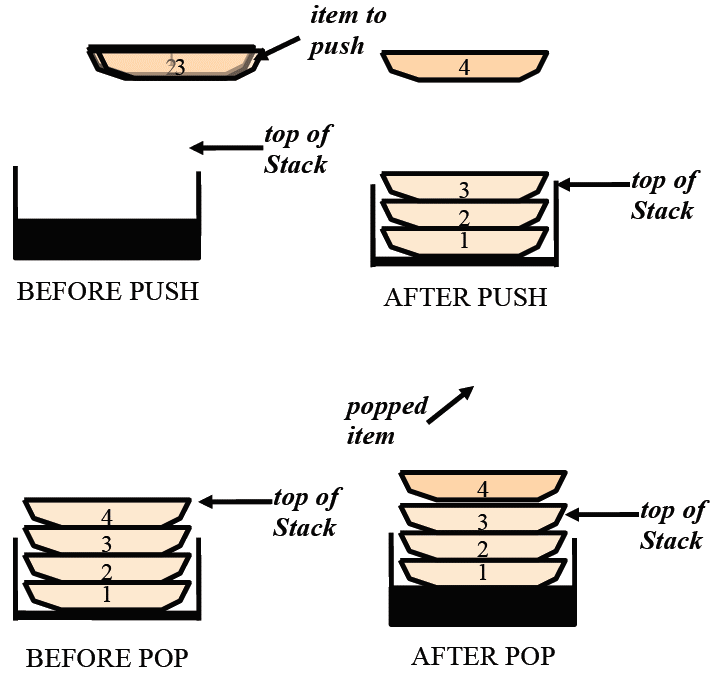
\includegraphics[width=0.55\textwidth]{figure/chap07/01stack02}
  \end{center}  
\end{frame}

\begin{frame}[t, fragile]{类模板的应用}{顺序堆栈类模板}%
  \begin{itemize}
  \item 类模板的定义    
  \end{itemize}
  \begin{center}
    \begin{tikzpicture}[font=\tiny, show background grid]
      \tikzset{coord/.style={coordinate}}

      \umlnote[text width=0.65\textwidth] (code1) at (0, 0)
      {
        \cppfilenobg{codes/chap07/08-stack-class.cpp}
      };
      
    \end{tikzpicture}
  \end{center}
\end{frame}

\begin{frame}[t, fragile]{类模板的应用}{顺序堆栈类模板}
  \begin{itemize}
  \item 类模板的函数模板
  \end{itemize}
  \begin{center}
    \begin{tikzpicture}[font=\tiny, show background grid]
      \tikzset{coord/.style={coordinate}}

      \umlnote[text width=0.4\textwidth] (code1) at (0, 0)
      {
        \cppfilenobg{codes/chap07/08-stack-fun-push.cpp}
      };

      \umlnote[text width=0.4\textwidth, right=0.3 of code1] (code2)
      {
        \cppfilenobg{codes/chap07/08-stack-fun-pop.cpp}
      };      
    \end{tikzpicture}
  \end{center}  
\end{frame}

\begin{frame}[t, fragile]{类模板的应用}{顺序堆栈类模板}%
  \begin{itemize}
  \item 类模板的使用
  \end{itemize}
  \begin{center}
    \begin{tikzpicture}[font=\tiny, show background grid]
      \tikzset{ coord/.style={coordinate} }
     
      \umlnote[text width=0.65\textwidth](code1)
      {
        \cppfilenobg{codes/chap07/08-stack-main.cpp}
      };

      \path let \p1=(code1) in
      coordinate (org) at (\x1, \y1)
      coordinate (ovBL11) at ($(org) + (-4.00, -0.35)$)
      coordinate (ovUR11) at ($(ovBL11) + (4.45, 1.55)$)
      coordinate (ovBR11) at ($(ovBL11) + (4.45, 0.00)$)
      coordinate (ovMR11) at ($(ovUR11)!0.5!(ovBR11)$)
      ;
      \path let \p1=(code1) in
      coordinate (org) at (\x1, \y1)
      coordinate (ovBL12) at ($(org) + (-4.00, -2.17)$)
      coordinate (ovUR12) at ($(ovBL12) + (5.00, 1.60)$)
      coordinate (ovBR12) at ($(ovBL12) + (5.00, 0.00)$)
      coordinate (ovMR12) at ($(ovUR12)!0.5!(ovBR12)$)
      ;

      \node[fill=blue!25, draw, xshift=-0.8cm, below=-0.2 of ovMR11]
      (note1) {字符栈};
      \node[fill=blue!25, draw, xshift=-0.9cm, below=-0.2 of ovMR12]
      (note2) {浮点数栈};
      
      \draw[red,thick,fill=green!35, fill opacity=0.3](ovBL11) rectangle
      (ovUR11);
      \draw[red,thick,fill=green!35, fill opacity=0.3](ovBL12) rectangle
      (ovUR12);      
    \end{tikzpicture}
  \end{center}
\end{frame}

\begin{frame}[t, fragile]{类模板的应用}{顺序堆栈类模板}%
  \begin{spacing}{1.8}
  \begin{itemize}
  \item 类模板成员函数声明与定义(实现)需处于同一文件。
  \item 分离编译模式:\cppinline{export}关键字
    \begin{itemize}
    \item VC与GCC编译器不支持
    \end{itemize}
  \item 其它解决方案\\[2ex]
    \tiny \url{http://www.codeproject.com/KB/cpp/Template_implementaion.aspx}
  \end{itemize}
  \end{spacing}
\end{frame}

\begin{frame}[t, fragile]{类模板的应用}{类模板的优缺点}%
  \begin{spacing}{1.8}
  \begin{itemize}
  \item 优势
    \begin{itemize}
    \item 通过数据类型参数化实现代码重用(设计一个类模板,可用于多种
      数据类型场合)
    \item STL的基础
    \end{itemize}
  \item 缺点
    \begin{itemize}
    \item 类层次上再次抽象,对初学者来说可读性较差,不易使用
    \end{itemize}
  \end{itemize}
  \end{spacing}
\end{frame}

%%%%%%%%%%%%%%%%%%%%%%%%%%%%%%%%%%%%%%%%%%%%%%%%%%%%%%%%%%%%%%%%
\section[STL]{STL编程}\label{sec:chap07-sec03}
\subsection[简介]{STL简介}\label{sec:chap07-sec03-01}
%%%%%%%%%%%%%%%%%%%%%%%%%%%%%%%%%%%%%%%%%%%%%%%%%%%%%%%%%%%%%%%%
\begin{frame}[t, fragile]{STL}{STL简介}%
  \begin{spacing}{1.8}
  \begin{itemize}
  \item 使用函数模板和类模板实现(类型参数化)
  \item 提供标准的数据结构和算法
  \item 可提高程序开发效率
  \end{itemize}
  \begin{center}
    
\includegraphics[width=0.4\textwidth]{figure/chap07/02stl01}
  \end{center}
  \end{spacing}
\end{frame}

\begin{frame}[t, fragile]{STL}{STL简介}%
  \begin{spacing}{1.4}
  \begin{itemize}
  \item 对初学者来说,语法晦涩难懂
  \item STL函数较多,不易记忆
  \item 建议:耐心学习参考例程
  \item 多看多练:\\
    \vspace{1em}
    \tiny
    \url{http://msdn.microsoft.com/en-us/library/c191tb28.aspx}\\
    \vspace{1em}
    \tiny \url{http://www.cplusplus.com/reference/stl/}
  \end{itemize}
  \begin{center}
    
\includegraphics[width=0.25\textwidth]{figure/chap07/02stl02}
  \end{center}
  \end{spacing}
\end{frame}

\begin{frame}[t, fragile]{STL}{STL简介}%
  \begin{spacing}{1.6}
  \begin{itemize}
  \item 组成(六部分)
    \begin{itemize}
    \item \alert{容器(Containers) }
    \item \alert{迭代器(Iterators) }
    \item \alert{算法(Algorithms)}
    \item 适配器(Adapters)
    \item 函数对象(Function Objects)
    \item 分配器(Allocators)
    \end{itemize}
  \end{itemize}
  \begin{center}
    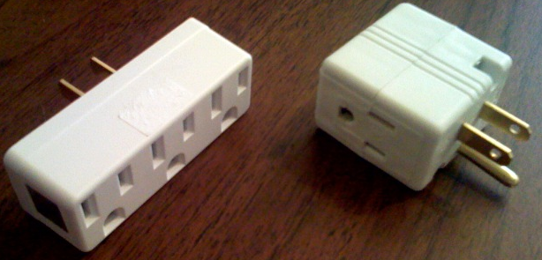
\includegraphics[width=0.4\textwidth]{figure/chap07/02stl03}
  \end{center}
  \end{spacing}
\end{frame}

\begin{frame}[t, fragile]{STL}{STL简介}%
  \begin{itemize}
  \item 组成(六部分)   
  \end{itemize}
  \begin{center}
    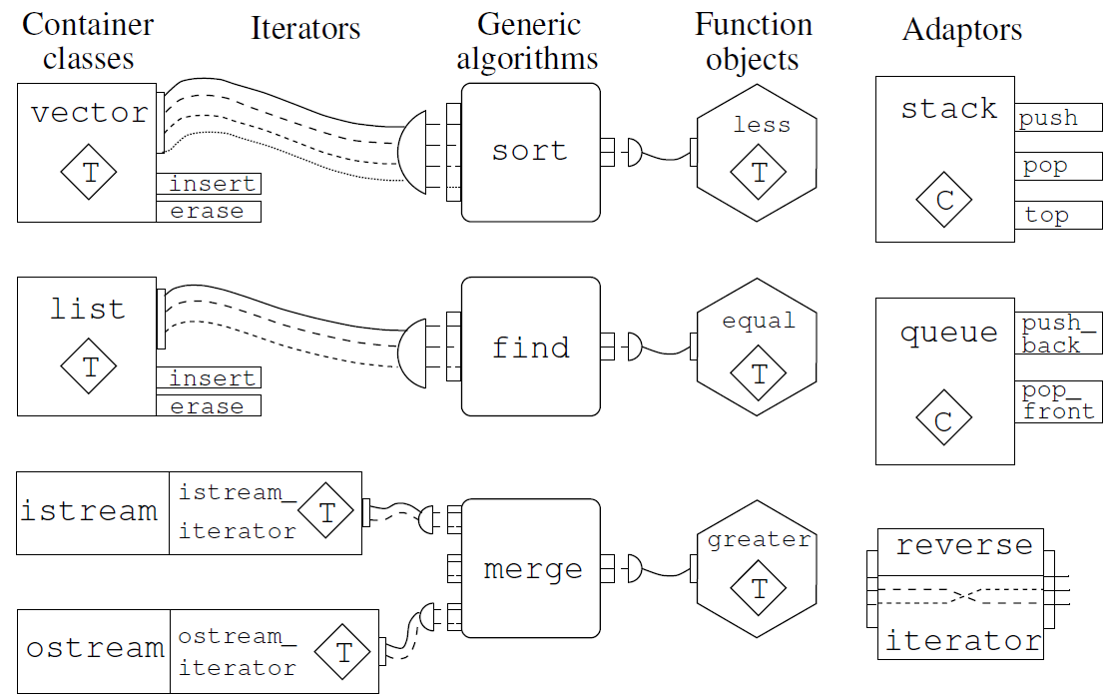
\includegraphics[width=0.75\textwidth]{figure/chap07/02stl04}
  \end{center}  
\end{frame}
%%%%%%%%%%%%%%%%%%%%%%%%%%%%%%%%%%%%%%%%%%%%%%%%%%%%%%%%%%%%%%%%

\subsection[容器]{STL容器}\label{sec:chap07-sec03-02}
%%%%%%%%%%%%%%%%%%%%%%%%%%%%%%%%%%%%%%%%%%%%%%%%%%%%%%%%%%%%%%%%
\begin{frame}[t, fragile]{容器}{容器简介}%
  \begin{itemize}
  \item 一个通用的数据结构
    \begin{itemize}
    \item 可以处理不同数据类型
    \item 包含基本的数据结构,如链表、堆栈、队列等
    \end{itemize}
  \end{itemize}
  \begin{center}
    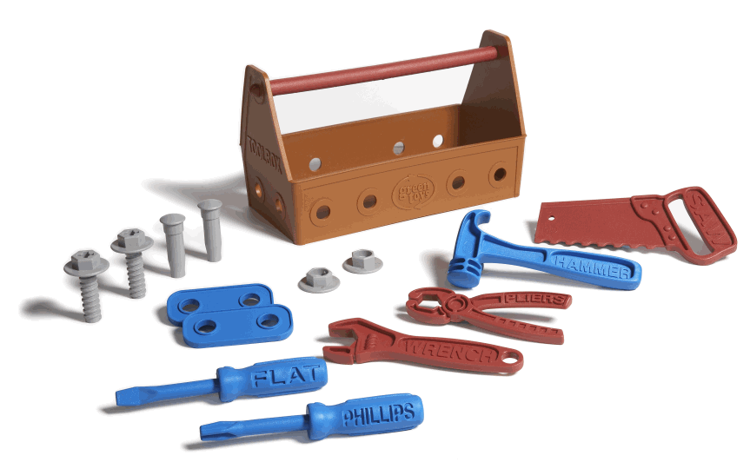
\includegraphics[width=0.75\textwidth]{figure/chap07/03stl05}    
  \end{center}  
\end{frame}

\begin{frame}[t, fragile]{容器}{容器分类}%
  \begin{itemize}
  \item 分类
    \begin{itemize}
    \item 顺序容器(sequence)
    \item 关联容器(sorted associative)
    \item 容器适配器(adaptors)
    \item 特殊容器(special)
    \end{itemize}
  \end{itemize}
  \begin{center}
    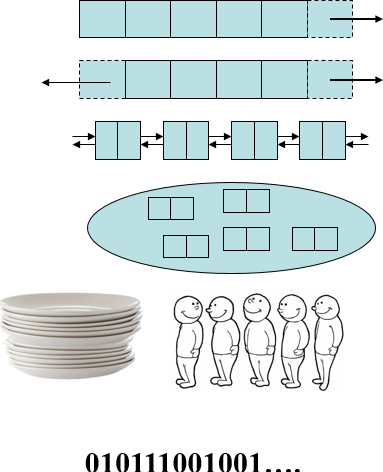
\includegraphics[width=0.4\textwidth]{figure/chap07/04stl0container}
  \end{center}  
\end{frame}

\begin{frame}[t, fragile]{容器}{顺序容器}%
  \stretchon
  \begin{itemize}
  \item 特点:添加或插入\alert{位置}与元素值无关(无自动排序)
    \begin{itemize}
    \item 向量(动态数组vector)\\
      \begin{tikzpicture}[scale=0.8,font=\tiny,x=0.5cm, y=0.5cm]
        \foreach \x in {0,1,...,8}
        {
          \node[inner sep=1pt] (BL\x) at (\x, 0) {};
          \node[inner sep=1pt] (UR\x) at (\x+1, 1) {};
          \node (MM\x) at ($(BL\x)!0.5!(UR\x)$) {};
        }
        \foreach \x in {0,1,...,5}
        {
          \draw[fill=green!25] (BL\x) rectangle (UR\x);
        }
        \draw[fill=green!25, dashed] (BL6) rectangle (UR6);   
        \draw[-{Stealth[scale=1.0]}, red, thick] (MM6) -- (MM8);        
      \end{tikzpicture}
    \item 列表(双向链表list)\\
      \begin{tikzpicture}[scale=0.8,font=\tiny,x=0.5cm, y=0.5cm]
        \foreach \x in {0,1,...,13}
        {          
          \node[inner sep=1pt] (BL\x) at (\x, 0) {};
          \node[inner sep=1pt] (UR\x) at (\x+0.5, 1) {};
          \node[inner sep=1pt] (BR\x) at (\x+0.5, 0) {};
          \node (MM\x) at ($(BR\x)!0.5!(UR\x)$) {};
        }        
        \foreach \x in {1,3,...,9}
        {
          \draw[fill=green!25] (BL\x) rectangle (UR\x);
          \draw[fill=green!25] ($(BL\x) + (0.5, 0)$) rectangle ($(UR\x) + (0.5, 0)$);
        }        
        \foreach \x in {0,2,...,10}
        {
          \draw[-{Stealth[scale=0.6]}, red, thick]
         ($(MM\x) + (-0.5, 0.15)$) -- ($(MM\x) + (0.5, 0.15)$);
          \draw[-{Stealth[scale=0.6]}, red, thick]
          ($(MM\x) + (0.5, -0.15)$) -- ($(MM\x) + (-0.5, -0.15)$);          
        }        
      \end{tikzpicture}
    \item 双端队列(deque: double-ended queue)\\
      \begin{tikzpicture}[scale=0.8,font=\tiny,x=0.5cm, y=0.5cm]
        \foreach \x in {0,1,...,9}
        {
          \node[inner sep=1pt] (BL\x) at (\x, 0) {};
          \node[inner sep=1pt] (UR\x) at (\x+1, 1) {};
          \node (MM\x) at ($(BL\x)!0.5!(UR\x)$) {};
        }
        \foreach \x in {3,4,...,6}
        {
          \draw[fill=green!25] (BL\x) rectangle (UR\x);
        }
        \draw[fill=green!25, dashed] (BL2) rectangle (UR2);
        \draw[fill=green!25, dashed] (BL7) rectangle (UR7);
        \draw[-{Stealth[scale=1.0]}, red, thick] (MM2) -- (MM0);
        \draw[-{Stealth[scale=1.0]}, red, thick] (MM7) -- (MM9);
      \end{tikzpicture}
    \end{itemize}
  \end{itemize}
  \stretchoff
\end{frame}

\begin{frame}[t, fragile]{容器}{时间复杂度}%
  \begin{spacing}{1.8}
  \begin{itemize}
  \item 注意:不同容器的插入、删除和存取特性不同,需根据任务选择合适
    容器
  \item 评价指标之一:\alert{时间复杂度}\\
    \centering
    \vspace{2em}
    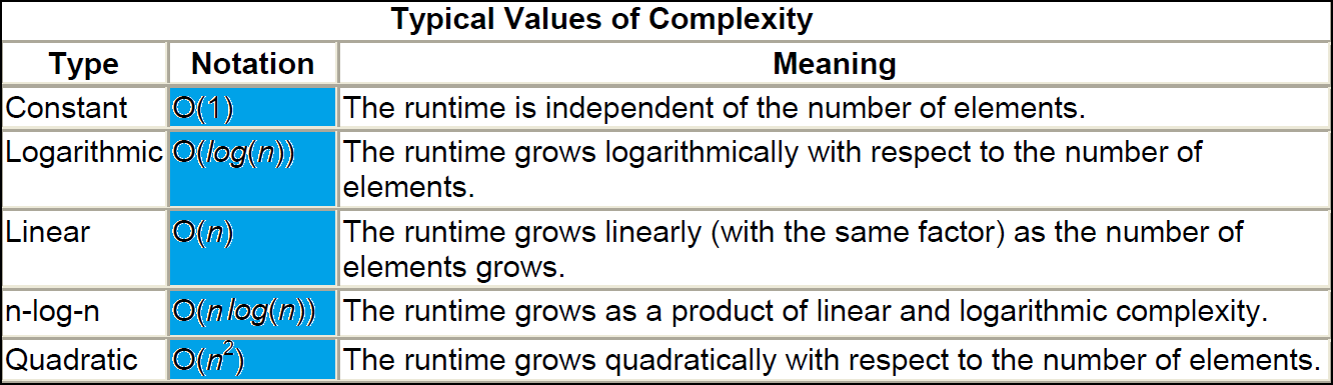
\includegraphics[width=0.75\textwidth]{figure/chap07/05stltimeO}    
  \end{itemize}
  \end{spacing}
\end{frame}

\begin{frame}[t, fragile]{容器}{向量容器(vector)}%
  \stretchon
  \begin{itemize}
  \item 特点\\
    \centering
    \begin{tikzpicture}[scale=0.8,font=\tiny,x=0.5cm, y=0.5cm]
        \foreach \x in {0,1,...,8}
        {
          \node[inner sep=1pt] (BL\x) at (\x, 0) {};
          \node[inner sep=1pt] (UR\x) at (\x+1, 1) {};
          \node (MM\x) at ($(BL\x)!0.5!(UR\x)$) {};
        }
        \foreach \x in {0,1,...,5}
        {
          \draw[fill=green!25] (BL\x) rectangle (UR\x);
        }
        \draw[fill=green!25, dashed] (BL6) rectangle (UR6);   
        \draw[-{Stealth[scale=1.0]}, red, thick] (MM6) -- (MM8);        
      \end{tikzpicture}
      \begin{itemize}
      \item 在内存中占有一块连续的空间(动态数组)
      \item 可自动扩充,且提供越界检查
      \item 适合在向量末尾插入或删除数据
      \item 可用[]运算符直接存取数据(随机访问random access)
      \end{itemize}      
    \end{itemize}
    \stretchoff
\end{frame}

\begin{frame}[t, fragile]{容器}{向量容器(vector)}%
  \begin{itemize}
  \item 例1 
  \end{itemize}
  \begin{center}
    \begin{tikzpicture}[font=\tiny, show background grid]
      \tikzset{coord/.style={coordinate}}

      \umlnote[text width=0.5\textwidth] (code1) at (0, 0)
      {
        \cppfilenobg{codes/chap07/09-vector01.cpp}
      };

      \path let \p1=(code1) in
      coordinate (org) at (\x1, \y1)
      coordinate (ovBL1) at ($(org) + (-3.30, 1.85)$)
      coordinate (ovUR1) at ($(ovBL1) + (1.85, 0.25)$)
      ;

      \path let \p1=(code1) in
      coordinate (org) at (\x1, \y1)
      coordinate (ovBL2) at ($(org) + (-3.00, 0.33)$)
      coordinate (ovUR2) at ($(ovBL2) + (1.52, 0.25)$)
      ;

      \path let \p1=(code1) in
      coordinate (org) at (\x1, \y1)
      coordinate (ovBL3) at ($(org) + (-2.75, -0.46)$)
      coordinate (ovUR3) at ($(ovBL3) + (1.65, 0.25)$)
      ;

      \path let \p1=(code1) in
      coordinate (org) at (\x1, \y1)
      coordinate (ovBL4) at ($(org) + (-2.75, -1.22)$)
      coordinate (ovUR4) at ($(ovBL4) + (1.45, 0.25)$)
      ;

      \path let \p1=(code1) in
      coordinate (org) at (\x1, \y1)
      coordinate (ovBL5) at ($(org) + (-0.60, -1.74)$)
      coordinate (ovUR5) at ($(ovBL5) + (0.95, 0.25)$)
      ;

      \path let \p1=(code1) in
      coordinate (org) at (\x1, \y1)
      coordinate (ovBL6) at ($(org) + (-1.95, -2.00)$)
      coordinate (ovUR6) at ($(ovBL6) + (0.50, 0.25)$)
      ;

      \draw[red,thick,fill=green!35, fill opacity=0.3](ovBL1) rectangle
      (ovUR1);

      \draw[green, thick, fill=green!25, fill opacity=0.3] (ovBL2)
      rectangle (ovUR2);

      \draw[blue, thick, fill=red!25, fill opacity=0.3] (ovBL3)
      rectangle (ovUR3);
      \draw[blue, thick, fill=red!25, fill opacity=0.3] (ovBL4)
      rectangle (ovUR4);
      \draw[blue, thick, fill=red!25, fill opacity=0.3] (ovBL5)
      rectangle (ovUR5);
      \draw[blue, thick, fill=red!25, fill opacity=0.3] (ovBL6)
      rectangle (ovUR6);      
    \end{tikzpicture}
  \end{center}
\end{frame}

\begin{frame}[t, fragile]{容器}{向量容器(vector)}%
  \begin{itemize}
  \item 例2 
  \end{itemize}
  \begin{center}
    \begin{tikzpicture}[font=\tiny, show background grid]
      \tikzset{coord/.style={coordinate}}

      \umlnote[text width=0.45\textwidth] (code1) at (0, 0)
      {
        \cppfilenobg{codes/chap07/09-vector02.cpp}
      };

      \path let \p1=(code1) in
      coordinate (org) at (\x1, \y1)
      coordinate (ovBL1) at ($(org) + (-2.98, 1.75)$)
      coordinate (ovUR1) at ($(ovBL1) + (1.85, 0.25)$)
      ;

      \path let \p1=(code1) in
      coordinate (org) at (\x1, \y1)
      coordinate (ovBL2) at ($(org) + (-2.70, 0.20)$)
      coordinate (ovUR2) at ($(ovBL2) + (2.05, 0.25)$)
      coordinate (ovBR2) at ($(ovBL2) + (2.05, 0.00)$)
      coordinate (ovMR2) at ($(ovBR2)!0.5!(ovUR2)$)
      ;

      % \path let \p1=(code1) in
      % coordinate (org) at (\x1, \y1)
      % coordinate (ovBL3) at ($(org) + (-3.4, -1.55)$)
      % coordinate (ovUR3) at ($(ovBL3) + (0.85, 0.25)$)
      % ;

      \node[fill=blue!25, draw, right=1.5 of ovMR2]
      (note1) {容量为6, 用1初始化};

      \draw[red,thick,fill=green!35, fill opacity=0.3](ovBL1) rectangle
      (ovUR1);

      \draw[green, thick, fill=green!25, fill opacity=0.3] (ovBL2)
      rectangle (ovUR2);

      % \draw[blue, thick, fill=red!25, fill opacity=0.3] (ovBL3)
      % rectangle (ovUR3);

      \draw[-{Stealth[scale=1.0]}, red, thick] (ovMR2.east) to [out =
      0, in = 180] (note1.west);
    \end{tikzpicture}
  \end{center}
\end{frame}

\begin{frame}[t, fragile]{容器}{向量容器(vector)}%
  \stretchon
  \begin{itemize}
  \item 复杂度\\
    \begin{tikzpicture}[scale=0.8,font=\tiny,x=0.5cm, y=0.5cm]
      \foreach \x in {0,1,...,8}
      {
        \node[inner sep=1pt] (BL\x) at (\x, 0) {};
        \node[inner sep=1pt] (UR\x) at (\x+1, 1) {};
        \node (MM\x) at ($(BL\x)!0.5!(UR\x)$) {};
      }

      \foreach \x in {0,1,...,5}
      {
        \draw[fill=green!25] (BL\x) rectangle (UR\x);
      }
      
      \draw[fill=green!25, dashed] (BL6) rectangle (UR6);
      \draw[-{Stealth[scale=1.0]}, red, thick] (MM6) -- (MM8);
    \end{tikzpicture}
    \begin{itemize}
    \item 随机存取:$O(1)$
    \item 向量末尾插入或删除:$O(1)$
    \end{itemize}
  \item 使用
    \begin{itemize}
    \item \cppinttfts{#include <vector>}
    \item 适于快速存取数据但非尾部频繁插入删除的场合
    \end{itemize}
  \end{itemize}
  \stretchoff
\end{frame}

\begin{frame}[t, fragile]{容器}{列表容器(list)}%
  \stretchon
  \begin{itemize}
  \item 特点\\
    \begin{tikzpicture}[scale=0.8,font=\tiny,x=0.5cm, y=0.5cm]
        \foreach \x in {0,1,...,13}
        {          
          \node[inner sep=1pt] (BL\x) at (\x, 0) {};
          \node[inner sep=1pt] (UR\x) at (\x+0.5, 1) {};
          \node[inner sep=1pt] (BR\x) at (\x+0.5, 0) {};
          \node (MM\x) at ($(BR\x)!0.5!(UR\x)$) {};
        }        
        \foreach \x in {1,3,...,9}
        {
          \draw[fill=green!25] (BL\x) rectangle (UR\x);
          \draw[fill=green!25] ($(BL\x) + (0.5, 0)$) rectangle ($(UR\x) + (0.5, 0)$);
        }        
        \foreach \x in {0,2,...,10}
        {
          \draw[-{Stealth[scale=0.6]}, red, thick]
         ($(MM\x) + (-0.5, 0.15)$) -- ($(MM\x) + (0.5, 0.15)$);
          \draw[-{Stealth[scale=0.6]}, red, thick]
          ($(MM\x) + (0.5, -0.15)$) -- ($(MM\x) + (-0.5, -0.15)$);          
        }        
    \end{tikzpicture}    
    \begin{itemize}
    \item 双向链表(前驱和后继)
    \item 可在任意位置插入或删除数据
    \item 不能用\cppinttfts{[]}运算符直接存取数据(不支持随机访问random access)
    \end{itemize}
  \end{itemize}
  \stretchoff
\end{frame}

\begin{frame}[t, fragile]{容器}{列表容器(list)}%
  \begin{itemize}
  \item 例3 
  \end{itemize}
  \vspace{-4ex}
  \begin{center}
    \begin{tikzpicture}[font=\tiny, show background grid]
      \tikzset{coord/.style={coordinate}}

      \umlnote[scale=0.9, text width=0.60\textwidth] (code1) at (0, 0)
      {
        \cppfilenobg{codes/chap07/10-list01.cpp}
      };

      \path let \p1=(code1) in
      coordinate (org) at (\x1, \y1)
      coordinate (ovBL1) at ($(org) + (-3.58, 2.2)$)
      coordinate (ovUR1) at ($(ovBL1) + (1.8, 0.5)$)
      ;

      \path let \p1=(code1) in
      coordinate (org) at (\x1, \y1)
      coordinate (ovBL2) at ($(org) + (-3.32, 1.52)$)
      coordinate (ovUR2) at ($(ovBL2) + (1.8, 0.25)$)
      ;

      \path let \p1=(code1) in
      coordinate (org) at (\x1, \y1)
      coordinate (ovBL3) at ($(org) + (-3.32, 1.08)$)
      coordinate (ovUR3) at ($(ovBL3) + (2.35, 0.25)$)
      coordinate (ovBR3) at ($(ovBL3) + (2.35, 0.0)$)
      coordinate (ovMR3) at ($(ovBR3)!0.5!(ovUR3)$)
      ;

      \path let \p1=(code1) in
      coordinate (org) at (\x1, \y1)
      coordinate (ovBL4) at ($(org) + (-3.32, -0.08)$)
      coordinate (ovUR4) at ($(ovBL4) + (2.1, 0.5)$)
      coordinate (ovBR4) at ($(ovBL4) + (2.1, 0.0)$)
      coordinate (ovMR4) at ($(ovBR4)!0.5!(ovUR4)$)
      ;

      \path let \p1=(code1) in
      coordinate (org) at (\x1, \y1)
      coordinate (ovBL5) at ($(org) + (-3.32, -0.75)$)
      coordinate (ovUR5) at ($(ovBL5) + (2.5, 0.5)$)
      ;

      \path let \p1=(code1) in
      coordinate (org) at (\x1, \y1)
      coordinate (ovBL6) at ($(org) + (-3.32, -1.90)$)
      coordinate (ovUR6) at ($(ovBL6) + (5.3, 0.25)$)
      ;

      \node[fill=blue!25, draw, right=2.5 of ovMR3]
      (note1) {迭代器:类似于指针};

      \draw[red,thick,fill=green!35, fill opacity=0.3](ovBL1) rectangle
      (ovUR1);

      \draw[green, thick, fill=green!25, fill opacity=0.3] (ovBL2)
      rectangle (ovUR2);

      \draw[red, thick, fill=red!25, fill opacity=0.3] (ovBL3)
      rectangle (ovUR3);
      \draw[red, thick, fill=red!25, fill opacity=0.3] (ovBL4)
      rectangle (ovUR4);
      \draw[blue, thick, fill=red!25, fill opacity=0.3] (ovBL5)
      rectangle (ovUR5);
      \draw[blue, thick, fill=red!25, fill opacity=0.3] (ovBL6)
      rectangle (ovUR6);

      \draw[-{Stealth[scale=1.0]}, red, thick] (ovMR3.east) to [out =
      0, in = 180] (note1.west);
      \draw[-{Stealth[scale=1.0]}, red, thick] (ovMR4.east) to [out =
      0, in = -135] (note1.south);
    \end{tikzpicture}
  \end{center}
\end{frame}

\begin{frame}[t, fragile]{容器}{列表容器(list)}%
  \begin{itemize}
  \item 例4 
  \end{itemize}
  \vspace{-4ex}
  \begin{center}
    \begin{tikzpicture}[font=\tiny, show background grid]
      \tikzset{coord/.style={coordinate}}

      \umlnote[scale=0.8, text width=0.60\textwidth] (code1) at (0, 0)
      {
        \cppfilenobg{codes/chap07/11-list02.cpp}
      };

      \path let \p1=(code1) in
      coordinate (org) at (\x1, \y1)
      coordinate (ovBL1) at ($(org) + (-3.2, 2.62)$)
      coordinate (ovUR1) at ($(ovBL1) + (1.45, 0.25)$)
      ;

      \path let \p1=(code1) in
      coordinate (org) at (\x1, \y1)
      coordinate (ovBL2) at ($(org) + (-2.95, 1.37)$)
      coordinate (ovUR2) at ($(ovBL2) + (2.35, 0.25)$)
      coordinate (ovBR2) at ($(ovBL2) + (2.35, 0.0)$)
      coordinate (ovMR2) at ($(ovBR2)!0.5!(ovUR2)$)
      ;

      \path let \p1=(code1) in
      coordinate (org) at (\x1, \y1)
      coordinate (ovBL3) at ($(org) + (-2.95, -0.96)$)
      coordinate (ovUR3) at ($(ovBL3) + (1.25, 0.5)$)
      coordinate (ovBR3) at ($(ovBL3) + (1.25, 0.0)$)
      coordinate (ovMR3) at ($(ovBR3)!0.5!(ovUR3)$)
      ;

      \path let \p1=(code1) in
      coordinate (org) at (\x1, \y1)
      coordinate (ovBL4) at ($(org) + (-2.95, -1.34)$)
      coordinate (ovUR4) at ($(ovBL4) + (1.8, 0.25)$)
      coordinate (ovBR4) at ($(ovBL4) + (1.8, 0.0)$)
      coordinate (ovMR4) at ($(ovBR4)!0.5!(ovUR4)$)
      ;
      \path let \p1=(code1) in
      coordinate (org) at (\x1, \y1)
      coordinate (ovBL5) at ($(org) + (-2.95, -2.15)$)
      coordinate (ovUR5) at ($(ovBL5) + (3.05, 0.25)$)
      coordinate (ovBR5) at ($(ovBL5) + (3.05, 0.0)$)
      coordinate (ovMR5) at ($(ovBR5)!0.5!(ovUR5)$)
      ;

      \node[fill=blue!25, draw, right=1.5 of ovMR2]
      (note1) {声明对象};
      \node[fill=blue!25, draw, right=1.5 of ovMR3]
      (note2) {排序};
      \node[fill=blue!25, draw, right=1.5 of ovMR4]
      (note3) {合并};

      \draw[red,thick,fill=green!35, fill opacity=0.3](ovBL1) rectangle
      (ovUR1);

      \draw[green, thick, fill=green!25, fill opacity=0.3] (ovBL2)
      rectangle (ovUR2);

      \draw[blue, thick, fill=red!25, fill opacity=0.3] (ovBL3)
      rectangle (ovUR3);
      \draw[blue, thick, fill=red!25, fill opacity=0.3] (ovBL4)
      rectangle (ovUR4);
      \draw[blue, thick, fill=red!25, fill opacity=0.3] (ovBL5)
      rectangle (ovUR5);

      \draw[-{Stealth[scale=1.0]}, red, thick] (ovMR2.east) to [out =
      0, in = 180] (note1.west);
      \draw[-{Stealth[scale=1.0]}, red, thick] (ovMR3.east) to [out =
      0, in = 180] (note2.west);
      \draw[-{Stealth[scale=1.0]}, red, thick] (ovMR4.east) to [out =
      0, in = 180] (note3.west);
      \draw[-{Stealth[scale=1.0]}, red, thick] (ovMR5.east) to [out =
      0, in = -135] (note3.south);
    \end{tikzpicture}
  \end{center}
\end{frame}

\begin{frame}[t, fragile]{容器}{列表容器(list)}%
  \stretchon
  \begin{itemize}
  \item 复杂度\\
    \begin{tikzpicture}[scale=0.8,font=\tiny,x=0.5cm, y=0.5cm]
        \foreach \x in {0,1,...,13}
        {          
          \node[inner sep=1pt] (BL\x) at (\x, 0) {};
          \node[inner sep=1pt] (UR\x) at (\x+0.5, 1) {};
          \node[inner sep=1pt] (BR\x) at (\x+0.5, 0) {};
          \node (MM\x) at ($(BR\x)!0.5!(UR\x)$) {};
        }        
        \foreach \x in {1,3,...,9}
        {
          \draw[fill=green!25] (BL\x) rectangle (UR\x);
          \draw[fill=green!25] ($(BL\x) + (0.5, 0)$) rectangle ($(UR\x) + (0.5, 0)$);
        }        
        \foreach \x in {0,2,...,10}
        {
          \draw[-{Stealth[scale=0.6]}, red, thick]
         ($(MM\x) + (-0.5, 0.15)$) -- ($(MM\x) + (0.5, 0.15)$);
          \draw[-{Stealth[scale=0.6]}, red, thick]
          ($(MM\x) + (0.5, -0.15)$) -- ($(MM\x) + (-0.5, -0.15)$);          
        }        
    \end{tikzpicture}    
    \begin{itemize}
    \item 访问前驱或后继:$O(1)$
    \item 根据索引值访问节点数据:$O(n)$
    \item 任意位置插入或删除:$O(1)$
    \end{itemize}
  \item 使用
    \begin{itemize}
    \item \cppinttfts{#include <list>}
    \item 适于数据频繁插入删除而不在意查找速度的场合
    \item 排序、合并操作效率高
    \end{itemize}
  \end{itemize}
  \stretchoff
\end{frame}

\begin{frame}[t, fragile]{容器}{双端队列容器(deque)}%
  \stretchon
  \begin{itemize}
  \item 特点\\
    \begin{tikzpicture}[scale=0.8,font=\tiny,x=0.5cm, y=0.5cm]
        \foreach \x in {0,1,...,9}
        {
          \node[inner sep=1pt] (BL\x) at (\x, 0) {};
          \node[inner sep=1pt] (UR\x) at (\x+1, 1) {};
          \node (MM\x) at ($(BL\x)!0.5!(UR\x)$) {};
        }
        \foreach \x in {3,4,...,6}
        {
          \draw[fill=green!25] (BL\x) rectangle (UR\x);
        }
        \draw[fill=green!25, dashed] (BL2) rectangle (UR2);
        \draw[fill=green!25, dashed] (BL7) rectangle (UR7);
        \draw[-{Stealth[scale=1.0]}, red, thick] (MM2) -- (MM0);
        \draw[-{Stealth[scale=1.0]}, red, thick] (MM7) -- (MM9);
    \end{tikzpicture}    
    \begin{itemize}
    \item 以多内存块(chunks of storage)形式存储数据
    \item 可自动扩充,且提供越界检查
    \item 适合在向量头尾插入或删除数据
    \item 可用\cppinttfts{[]}运算符直接存取数据(随机访问random access)
    \end{itemize}
  \end{itemize}
  \stretchoff
\end{frame}

\begin{frame}[t, fragile]{容器}{双端队列容器(deque)}%
  \begin{itemize}
  \item 例5 
  \end{itemize}
  \vspace{-2ex}
  \begin{center}
    \begin{tikzpicture}[font=\tiny, show background grid]
      \tikzset{coord/.style={coordinate}}

      \umlnote[scale=1.2, text width=0.60\textwidth] (code1) at (0, 0)
      {
        \cppfilenobg{codes/chap07/12-deque01.cpp}
      };

      \path let \p1=(code1) in
      coordinate (org) at (\x1, \y1)
      coordinate (ovBL1) at ($(org) + (-4.75, 1.92)$)
      coordinate (ovUR1) at ($(ovBL1) + (2.2, 0.3)$)
      ;

      \path let \p1=(code1) in
      coordinate (org) at (\x1, \y1)
      coordinate (ovBL2) at ($(org) + (-4.45, 0.40)$)
      coordinate (ovUR2) at ($(ovBL2) + (2.2, 0.3)$)
      ;

      \path let \p1=(code1) in
      coordinate (org) at (\x1, \y1)
      coordinate (ovBL3) at ($(org) + (-4.1, -0.84)$)
      coordinate (ovUR3) at ($(ovBL3) + (3.00, 0.3)$)
      ;

      \path let \p1=(code1) in
      coordinate (org) at (\x1, \y1)
      coordinate (ovBL4) at ($(org) + (-2.15, -1.77)$)
      coordinate (ovUR4) at ($(ovBL4) + (1.3, 0.3)$)
      ;

      \path let \p1=(code1) in
      coordinate (org) at (\x1, \y1)
      coordinate (ovBL5) at ($(org) + (-3.15, -2.07)$)
      coordinate (ovUR5) at ($(ovBL5) + (0.8, 0.3)$)
      ;
     
      \draw[red,thick,fill=green!35, fill opacity=0.3](ovBL1) rectangle
      (ovUR1);
      \draw[green, thick, fill=green!25, fill opacity=0.3] (ovBL2)
      rectangle (ovUR2);
      \draw[blue, thick, fill=red!25, fill opacity=0.3] (ovBL3)
      rectangle (ovUR3);
      \draw[blue, thick, fill=red!25, fill opacity=0.3] (ovBL4)
      rectangle (ovUR4);
      \draw[blue, thick, fill=red!25, fill opacity=0.3] (ovBL5)
      rectangle (ovUR5);      
    \end{tikzpicture}
  \end{center}
\end{frame}

\begin{frame}[t, fragile]{容器}{双端队列容器(deque)}%
  \begin{itemize}
  \item 例6 
  \end{itemize}
  \vspace{-4ex}
  \begin{center}
    \begin{tikzpicture}[font=\tiny, show background grid]
      \tikzset{coord/.style={coordinate}}

      \umlnote[scale=0.8, text width=0.60\textwidth] (code1) at (0, 0)
      {
        \cppfilenobg{codes/chap07/13-deque02.cpp}
      };

      \path let \p1=(code1) in
      coordinate (org) at (\x1, \y1)
      coordinate (ovBL1) at ($(org) + (-3.2, 2.60)$)
      coordinate (ovUR1) at ($(ovBL1) + (1.5, 0.25)$)
      ;

      \path let \p1=(code1) in
      coordinate (org) at (\x1, \y1)
      coordinate (ovBL2) at ($(org) + (-2.95, 1.16)$)
      coordinate (ovUR2) at ($(ovBL2) + (1.7, 0.25)$)
      coordinate (ovBR2) at ($(ovBL2) + (1.7, 0.0)$)
      coordinate (ovMR2) at ($(ovBR2)!0.5!(ovUR2)$)
      ;

      \path let \p1=(code1) in
      coordinate (org) at (\x1, \y1)
      coordinate (ovBL3) at ($(org) + (-2.95, 0.77)$)
      coordinate (ovUR3) at ($(ovBL3) + (2.7, 0.25)$)
      coordinate (ovBR3) at ($(ovBL3) + (2.7, 0.0)$)
      coordinate (ovMR3) at ($(ovBR3)!0.5!(ovUR3)$)
      ;

      \path let \p1=(code1) in
      coordinate (org) at (\x1, \y1)
      coordinate (ovBL4) at ($(org) + (-2.75, -1.72)$)
      coordinate (ovUR4) at ($(ovBL4) + (2.4, 0.25)$)
      coordinate (ovBR4) at ($(ovBL4) + (2.4, 0.0)$)
      coordinate (ovMR4) at ($(ovBR4)!0.5!(ovUR4)$)
      ;
      \path let \p1=(code1) in
      coordinate (org) at (\x1, \y1)
      coordinate (ovBL5) at ($(org) + (-2.95, -2.13)$)
      coordinate (ovUR5) at ($(ovBL5) + (2.5, 0.25)$)
      coordinate (ovBR5) at ($(ovBL5) + (2.5, 0.0)$)
      coordinate (ovMR5) at ($(ovBR5)!0.5!(ovUR5)$)
      ;

      \node[fill=blue!25, draw, right=1.5 of ovMR2]
      (note1) {声明对象};
      \node[fill=blue!25, draw, right=1.5 of ovMR3]
      (note2) {添加3个数据:Hello字符串};
      \node[fill=blue!25, draw, right=1.5 of ovMR4]
      (note3) {下标访问};
      \node[fill=blue!25, draw, right=1.5 of ovMR5]
      (note4) {扩展为4个元素, 扩展后的元素赋值为Hello C++};

      \draw[red,thick,fill=green!35, fill opacity=0.3](ovBL1) rectangle
      (ovUR1);

      \draw[green, thick, fill=green!25, fill opacity=0.3] (ovBL2)
      rectangle (ovUR2);

      \draw[blue, thick, fill=red!25, fill opacity=0.3] (ovBL3)
      rectangle (ovUR3);
      \draw[blue, thick, fill=red!25, fill opacity=0.3] (ovBL4)
      rectangle (ovUR4);
      \draw[blue, thick, fill=red!25, fill opacity=0.3] (ovBL5)
      rectangle (ovUR5);

      \draw[-{Stealth[scale=1.0]}, red, thick] (ovMR2.east) to [out =
      0, in = 180] (note1.west);
      \draw[-{Stealth[scale=1.0]}, red, thick] (ovMR3.east) to [out =
      0, in = 180] (note2.west);
      \draw[-{Stealth[scale=1.0]}, red, thick] (ovMR4.east) to [out =
      0, in = 180] (note3.west);
      \draw[-{Stealth[scale=1.0]}, red, thick] (ovMR5.east) to [out =
      0, in = 180] (note4.west);
    \end{tikzpicture}
  \end{center}
\end{frame}

\begin{frame}[t, fragile]{容器}{双端队列容器(deque)}%
  \stretchon
  \begin{itemize}
  \item 复杂度\\
    \begin{tikzpicture}[scale=0.8,font=\tiny,x=0.5cm, y=0.5cm]
        \foreach \x in {0,1,...,9}
        {
          \node[inner sep=1pt] (BL\x) at (\x, 0) {};
          \node[inner sep=1pt] (UR\x) at (\x+1, 1) {};
          \node (MM\x) at ($(BL\x)!0.5!(UR\x)$) {};
        }
        \foreach \x in {3,4,...,6}
        {
          \draw[fill=green!25] (BL\x) rectangle (UR\x);
        }
        \draw[fill=green!25, dashed] (BL2) rectangle (UR2);
        \draw[fill=green!25, dashed] (BL7) rectangle (UR7);
        \draw[-{Stealth[scale=1.0]}, red, thick] (MM2) -- (MM0);
        \draw[-{Stealth[scale=1.0]}, red, thick] (MM7) -- (MM9);
    \end{tikzpicture}  
    \begin{itemize}
    \item 随机存取:$O(1)$
    \item 队列头尾插入或删除:$O(1)$
    \end{itemize}
  \item 使用
    \begin{itemize}
    \item \cppinttfts{#include <deque>}
    \item 适于快速在队列头尾存取数据但非频繁插入删除的场合 
    \item 若非头尾插入删除数据,效率比list低
    \end{itemize}
  \end{itemize}
  \stretchoff
\end{frame}

\begin{frame}[t, fragile]{容器}{关联容器}%
  \stretchon
  \begin{itemize}
  \item 特点:元素的添加或插入位置与元素的值相关
    \begin{itemize}
    \item 集合(set)和多集(multiset,允许重复元素)
    \item 映射(map)和多映射(multimap,允许重复元素键值)
    \end{itemize}
  \item 复杂度:插入、删除和查找$O(log(n))$
  \end{itemize}
  \stretchoff
\end{frame}

\begin{frame}[t, fragile]{容器}{容器适配器}%
  \stretchon
  \begin{itemize}
  \item 由顺序容器转换出的新容器(list→queue, vector→stack),\alert{不支持迭
    代器}
    \begin{itemize}
    \item 队列(queue)
    \item 优先队列(priority queue)
    \item 堆栈(stack)
    \end{itemize}
  \end{itemize}
  \stretchoff
  \begin{center}
    
\includegraphics[height=0.23\textheight]{figure/chap07/06queue}
    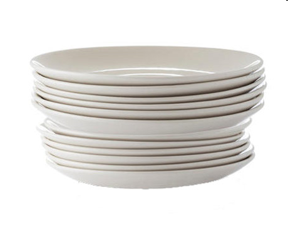
\includegraphics[height=0.23\textheight]{figure/chap07/07stack}
  \end{center}  
\end{frame}

\begin{frame}[t, fragile]{容器}{特殊容器}%
  \stretchon
  \begin{itemize}
  \item 位集bitset:灵活对二进制位进行操作
    \begin{itemize}
    \item 整型到二进制的转换
    \item 位的直接访问和设置等
    \end{itemize}
  \end{itemize}
  \stretchoff
\end{frame}
%%%%%%%%%%%%%%%%%%%%%%%%%%%%%%%%%%%%%%%%%%%%%%%%%%%%%%%%%%%%%%%%

\subsection[迭代器]{STL迭代器}\label{sec:chap07-sec03-03}
%%%%%%%%%%%%%%%%%%%%%%%%%%%%%%%%%%%%%%%%%%%%%%%%%%%%%%%%%%%%%%%%
\begin{frame}[t, fragile]{迭代器}{迭代器定义}%
  \stretchon
  \begin{itemize}
  \item 能对顺序容器或关联容器中的每个元素进行连续存取的对象(一个特殊
    的指针)
  \item 容器名\cppinlinett{<|数据类型|>::iterator} 迭代器名
  \item 非标准迭代器
    \begin{itemize}
    \item \cppinttfts{const_iterator}
    \item \cppinttfts{reverse_iterator}
    \item \cppinttfts{const_reverse_iterator}
    \end{itemize}
  \end{itemize}
  \stretchoff
\end{frame}

\begin{frame}[t, fragile]{迭代器}{迭代器定义}%
  \begin{itemize}
  \item \cppinlinett{|容器名|.begin()},\cppinlinett{|容器名|.end()}
  \item \cppinlinett{|容器名|.size()}
  \end{itemize}
  \begin{center}
    \begin{tikzpicture}[scale=0.8,font=\tiny,x=1.0cm, y=1.0cm]
        \foreach \x in {0,1,...,9}
        {
          \node[inner sep=1pt] (BL\x) at (\x, 0) {};
          \node[inner sep=1pt] (UR\x) at (\x+1, 1) {};
          \node (MM\x) at ($(BL\x)!0.5!(UR\x)$) {};
        }
        \foreach \x in {1,2,...,8}
        {
          \draw[fill=green!25] (BL\x) rectangle (UR\x);
        }
        \draw[fill=green!25, dashed] (BL0) rectangle (UR0);
        \draw[fill=green!25, dashed] (BL9) rectangle (UR9);

        \node[fill=green!75!yellow, draw, above=1.0 of MM1] (note1)
        {\large begin()};
        \node[fill=green!75!yellow, draw, above=1.0 of MM9] (note2)
        {\large end()};
        \node[fill=green!75!yellow, draw, below=1.0 of MM0] (note3)
        {\large rend()};
        \node[fill=green!75!yellow, draw, below=1.0 of MM8] (note4)
        {\large rbegin()};

        \draw[-{Stealth[scale=1.0]}, red, thick] (note1.south) --
        (MM1.north);
        \draw[-{Stealth[scale=1.0]}, red, thick] (note2.south) --
        (MM9.north);
        \draw[-{Stealth[scale=1.0]}, red, thick] (note3.north) --
        (MM0.south);
        \draw[-{Stealth[scale=1.0]}, red, thick] (note4.north) --
        (MM8.south);        
    \end{tikzpicture}
  \end{center}
\end{frame}

\begin{frame}[t, fragile]{迭代器}{迭代器定义}%
  \begin{itemize}
  \item 例7 
  \end{itemize}
  \begin{center}
    \begin{tikzpicture}[font=\tiny, show background grid]
      \tikzset{coord/.style={coordinate}}

      \umlnote[scale=1.2, text width=0.6\textwidth] (code1) at (0, 0)
      {
        \cppfilenobg{codes/chap07/14-iterator01.cpp}
      };

      \path let \p1=(code1) in
      coordinate (org) at (\x1, \y1)
      coordinate (ovBL1) at ($(org) + (-4.4, -0.53)$)
      coordinate (ovUR1) at ($(ovBL1) + (4.2, 0.3)$)
      ;

      \path let \p1=(code1) in
      coordinate (org) at (\x1, \y1)
      coordinate (ovBL2) at ($(org) + (-4.4, -2.05)$)
      coordinate (ovUR2) at ($(ovBL2) + (4.8, 0.3)$)
      coordinate (ovBR2) at ($(ovBL2) + (4.8, 0.0)$)
      coordinate (ovMR2) at ($(ovBR2)!0.5!(ovUR2)$)
      ;

      \path let \p1=(code1) in
      coordinate (org) at (\x1, \y1)
      coordinate (ovBL3) at ($(org) + (-3.15, -2.37)$)
      coordinate (ovUR3) at ($(ovBL3) + (0.4, 0.3)$)
      coordinate (ovBR3) at ($(ovBL3) + (0.4, 0.0)$)
      coordinate (ovMR3) at ($(ovBR3)!0.5!(ovUR3)$)
      ;

      \node[fill=blue!25, draw, yshift=1.0cm, right=1.0 of ovMR2]
      (note1) {\alert{非p--}};

      \draw[red,thick,fill=green!35, fill opacity=0.3](ovBL1) rectangle
      (ovUR1);
      \draw[blue, thick, fill=green!25, fill opacity=0.3] (ovBL2)
      rectangle (ovUR2);
      \draw[blue, thick, fill=red!25, fill opacity=0.3] (ovBL3)
      rectangle (ovUR3);

      \draw[-{Stealth[scale=1.0]}, red, thick] (note1.west) to [out =
      180, in = 0] (ovMR2.east);
    \end{tikzpicture}
  \end{center}
\end{frame}

\begin{frame}[t, fragile]{迭代器}{迭代器分类}%
  \begin{itemize}
  \item 分类 
  \end{itemize}
  \begin{center}
    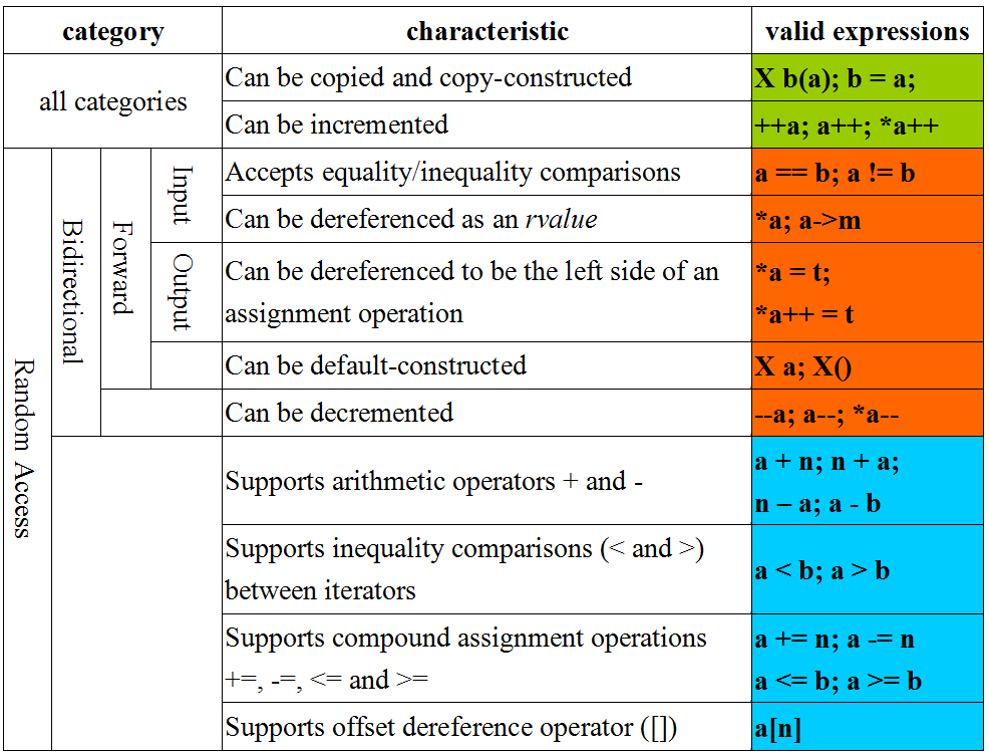
\includegraphics[width=0.65\textwidth]{figure/chap07/08iterator01}
  \end{center}
\end{frame}

\begin{frame}[t, fragile]{迭代器}{迭代器分类}%
  \stretchon
  \begin{itemize}
  \item 在vector和deque中实现跳跃式访问\\
    \begin{cppcode}
vector <int>::iterator p;
for(p=v.begin(); p!=v.end(); p+=2)
    \end{cppcode}
  \item list中使用“\cppinline{+=}”无法实现
    \begin{itemize}
    \item 使用函数advance\\
      \begin{cppcode}
list <int>::iterator p;
for(p=v.begin(); p!=v.end(); advance(p,2))
      \end{cppcode}
    \end{itemize}
  \item 提供一种\alert{一般化方法(generic method)}对\alert{不同类型容器}中的
      元素\alert{进行访问}
  \end{itemize}
  \stretchoff
\end{frame}

\begin{frame}[t, fragile]{迭代器}{迭代器的作用}%
  \begin{itemize}
  \item 迭代器示例
  \end{itemize}
  \begin{center}
    \begin{tikzpicture}[font=\tiny, show background grid]
      \tikzset{coord/.style={coordinate}}
      \umlnote[scale=0.9, text width=0.45\textwidth] (code1) at (0, 0)
      {
        \cppfilenobg{codes/chap07/15-itertempfind.cpp}
      };
      \umlnote[scale=0.9, text width=0.45\textwidth, below=0.2 of code1] (code2)
      {
        \cppfilenobg{codes/chap07/15-itertempprint.cpp}
      }; 
    \end{tikzpicture}
  \end{center}
\end{frame}

\begin{frame}[t, fragile]{迭代器}{迭代器的作用}%
  \begin{itemize}
  \item 迭代器示例
  \end{itemize}
  \begin{center}
    \begin{tikzpicture}[font=\tiny, show background grid]
      \tikzset{coord/.style={coordinate}}
      \umlnote[scale=0.9, text width=0.65\textwidth] (code1) at (0, 0)
      {
        \cppfilenobg{codes/chap07/15-itertempmain.cpp}
      };
    \end{tikzpicture}
  \end{center}
\end{frame}

%%%%%%%%%%%%%%%%%%%%%%%%%%%%%%%%%%%%%%%%%%%%%%%%%%%%%%%%%%%%%%%%
\subsection[算法]{STL算法}\label{sec:chap07-sec03-04}
%%%%%%%%%%%%%%%%%%%%%%%%%%%%%%%%%%%%%%%%%%%%%%%%%%%%%%%%%%%%%%%%
\begin{frame}[t, fragile]{算法}{简介}
  \stretchon
  \begin{itemize}
  \item 算法实现机理
  \item 非修改操作Non-modifying sequence operations
  \item 修改操作Modifying sequence operations
  \item 排序Sorting
  \item 堆Heap
  \item 二分查找Binary search
  \item 合并Merge
  \item 最小最大值Min/max
  \end{itemize}
  \stretchoff
\end{frame}

\begin{frame}[t, fragile]{算法}{实现机理}
  \stretchon
  \begin{itemize}
  \item 基于迭代器和函数模板
  \item 算法<algorithm>是用来处理一个数据序列区间(range)的函数集合
  \item 区间中的元素通过迭代器进行访问
  \item 独立于所操作的容器
  \end{itemize}
  \stretchoff
\end{frame}

\begin{frame}[t, fragile]{算法}{非修改操作}
  \begin{tabbing}
    \cppinline{for_each} \hspace{3em} \=  Apply function to range\\
    \cppinline{find} \> Find value in range\\ 
    \cppinline{find_if} \> Find element in range\\
    \cppinline{find_end} \> Find last subsequence in range\\
    \cppinline{find_first_of} \> Find element from set in range\\ 
    \cppinline{adjacent_find} \> Find equal adjacent elements in range\\ 
    \cppinline{count} \> Count appearances of value in range\\ 
    \cppinline{count_if} \> Return number of elements in range\\
                                    \> satisfying condition\\
    \cppinline{mismatch} \> Return first position where two ranges\\
                                       \> differ\\
    \cppinline{equal} \> Test whether the elements in two ranges\\
                                \>       are equal\\
    \cppinline{search} \> Find subsequence in range\\
    \cppinline{search_n} \> Find succession of equal values in range
  \end{tabbing}
\end{frame}

\begin{frame}[t, fragile]{算法}{非修改操作}
  \begin{itemize}
  \item \cppinline{find}函数模板
  \end{itemize}
  \begin{center}
    \begin{tikzpicture}[font=\tiny, show background grid]
      \tikzset{coord/.style={coordinate}}
      \umlnote[scale=1.0, text width=0.7\textwidth] (code1) at (0, 0)
      {
        \cppfilenobg{codes/chap07/16-find.cpp}
      };
    \end{tikzpicture}
  \end{center}
\end{frame}

\begin{frame}[t, fragile]{算法}{非修改操作}
  \begin{itemize}
  \item \cppinline{find}函数模板
  \end{itemize}
  \begin{center}
    \begin{tikzpicture}[font=\tiny, show background grid]
      \tikzset{coord/.style={coordinate}}
      \umlnote[scale=0.9, text width=0.65\textwidth] (code1) at (0, 0)
      {
        \cppfilenobg{codes/chap07/16-findexample.cpp}
      };
    \end{tikzpicture}
  \end{center}
\end{frame}

\begin{frame}[t, fragile]{算法}{非修改操作}
  \begin{itemize}
  \item \cppinline{for_each}函数模板
  \end{itemize}
  \begin{center}
    \begin{tikzpicture}[font=\tiny, show background grid]
      \tikzset{coord/.style={coordinate}}
      \umlnote[scale=1.0, text width=0.68\textwidth] (code1) at (0, 0)
      {
        \cppfilenobg{codes/chap07/17-foreach.cpp}
      };

      \path let \p1=(code1) in
      coordinate (org) at (\x1, \y1)
      coordinate (ovBL1) at ($(org) + (1.57, -0.08)$)
      coordinate (ovUR1) at ($(ovBL1) + (1.2, 0.26)$)
      coordinate (ovBR1) at ($(ovBL1) + (1.2, 0.0)$)
      coordinate (ovMB1) at ($(ovBL1)!0.5!(ovBR1)$)
      ;

      \node[fill=blue!25, draw, xshift=-2.0cm, below=1.8 of ovMB1]
      (note1) {\alert{函数指针}};
      \node[fill=blue!25, draw, xshift=1.5cm, below=1.8 of ovMB1]
      (note2) {\alert{函数对象}};

      \draw[red, thick, fill=green!35, fill opacity=0.3] (ovBL1)
      rectangle (ovUR1);
      
      \draw[-{Stealth[scale=1.0]}, red, thick] (ovMB1.south) to [out =
      -90, in = 90] (note1.north);
      \draw[-{Stealth[scale=1.0]}, red, thick] (ovMB1.south) to [out =
      -90, in = 90] (note2.north);      
    \end{tikzpicture}
  \end{center}
\end{frame}

\begin{frame}[t, fragile]{算法}{非修改操作}
  \begin{itemize}
  \item \cppinline{for_each}函数模板
  \end{itemize}
  \begin{center}
    \begin{tikzpicture}[font=\tiny, show background grid]
      \tikzset{coord/.style={coordinate}}
      \umlnote[scale=0.65, text width=0.65\textwidth] (code1) at (0, 0)
      {
        \cppfilenobg{codes/chap07/17-foreachexample.cpp}
      };
    \end{tikzpicture}
  \end{center}
\end{frame}

\begin{frame}[t, fragile]{算法}{非修改操作}
  \begin{itemize}
  \item \cppinline{count_if}函数模板
  \end{itemize}
  \begin{center}
    \begin{tikzpicture}[font=\tiny, show background grid]
      \tikzset{coord/.style={coordinate}}
      \umlnote[scale=1.0, text width=0.675\textwidth] (code1) at (0, 0)
      {
        \cppfilenobg{codes/chap07/18-counterif.cpp}
      };

      \path let \p1=(code1) in
      coordinate (org) at (\x1, \y1)
      coordinate (ovBL1) at ($(org) + (-4.5, 0.16)$)
      coordinate (ovUR1) at ($(ovBL1) + (2.62, 1.10)$)
      coordinate (ovBR1) at ($(ovBL1) + (2.62, 0.0)$)
      coordinate (ovMR1) at ($(ovUR1)!0.5!(ovBR1)$)
      ;

      \path let \p1=(code1) in
      coordinate (org) at (\x1, \y1)
      coordinate (ovBL2) at ($(org) + (-2.6, -2.10)$)
      coordinate (ovUR2) at ($(ovBL2) + (1.0, 0.25)$)
      ;

      \path let \p1=(code1) in
      coordinate (org) at (\x1, \y1)
      coordinate (ovBL3) at ($(org) + (0.5, -2.10)$)
      coordinate (ovUR3) at ($(ovBL3) + (0.62, 0.26)$)
      coordinate (ovUL3) at ($(ovBL3) + (0.0, 0.26)$)
      coordinate (ovMA3) at ($(ovUR3)!0.5!(ovUL3)$)
      ;

      \draw[red, thick, fill=green!35, fill opacity=0.3] (ovBL1)
      rectangle (ovUR1);
      \draw[blue, thick, fill=green!35, fill opacity=0.3] (ovBL2)
      rectangle (ovUR2);
      \draw[red, thick, fill=green!35, fill opacity=0.3] (ovBL3)
      rectangle (ovUR3);

      \draw[-{Stealth[scale=1.0]}, red, thick] (ovMA3.north) to [out =
      90, in = 0] (ovMR1.east);
    \end{tikzpicture}
  \end{center}
\end{frame}

\begin{frame}[t, fragile, allowframebreaks]{算法}{修改操作}
  \begin{tabbing}
    \cppinline{copy} \hspace{6em} \= Copy range of elements\\
    \cppinline{copy_backward} \> Copy range of elements backwards\\ 
    \cppinline{swap} \> Exchange values of two objects\\ 
    \cppinline{swap_ranges} \> Exchange values of two ranges\\ 
    \cppinline{iter_swap} \> Exchange values of objects pointed \\
                                      \> by two iterators\\ 
    \cppinline{transform} \> Apply function to range\\ 
    \cppinline{replace} \> Replace value in range\\ 
    \cppinline{replace_if} \> Replace values in range\\
    \cppinline{replace_copy} \> Copy range replacing value\\
    \cppinline{replace_copy_if} \> Copy range replacing value\\ 
    \cppinline{fill} \> Fill range with value\\ 
    \cppinline{fill_n} \> Fill sequence with value\\ 
    \cppinline{generate} \> Generate values for range with function\\ 
    \cppinline{generate_n} \> Generate values for sequence with function\\
    \cppinline{remove} \> Remove value from range\\ 
    \cppinline{remove_if} \> Remove elements from range\\ 
    \cppinline{remove_copy} \> Copy range removing value\\ 
    \cppinline{remove_copy_if} \> Copy range removing values\\ 
    \cppinline{unique} \> Remove consecutive duplicates in range\\ 
    \cppinline{unique_copy} \> Copy range removing duplicates\\ 
    \cppinline{reverse} \> Reverse range\\ 
    \cppinline{reverse_copy} \> Copy range reversed\\
    \cppinline{rotate} \> Rotate elements in range\\ 
    \cppinline{rotate_copy} \> Copy rotated range\\ 
    \cppinline{random_shuffle} \> Rearrange elements in range randomly\\ 
    \cppinline{partition} \> Partition range in two\\ 
    \cppinline{stable_partition} \> Partition range in two - stable ordering 
  \end{tabbing}
\end{frame}

\begin{frame}[t, fragile]{算法}{修改操作}
  \begin{itemize}
  \item 替换函数\cppinline{replace}
  \end{itemize}
  \begin{center}
    \begin{tikzpicture}[font=\tiny, show background grid]
      \tikzset{coord/.style={coordinate}}
      \umlnote[scale=0.95, text width=0.75\textwidth] (code1) at (0, 0)
      {
        \cppfilenobg{codes/chap07/19-replace.cpp}
      };
    \end{tikzpicture}
  \end{center}
\end{frame}

\begin{frame}[t, fragile]{算法}{修改操作}
  \begin{itemize}
  \item 删除函数\cppinline{remove}
  \end{itemize}
  \begin{center}
    \begin{tikzpicture}[font=\tiny, show background grid]
      \tikzset{coord/.style={coordinate}}
      \umlnote[scale=1.0, text width=0.75\textwidth] (code1) at (0, 0)
      {
        \cppfilenobg{codes/chap07/20-remove.cpp}
      };
    \end{tikzpicture}
  \end{center}
\end{frame}

\begin{frame}[t, fragile, allowframebreaks]{算法}{修改操作}
  \begin{itemize}
  \item 排序算法
  \end{itemize}
  \begin{tabbing}
    \cppinline{sort} \hspace{9em} \= Sort elements in range\\
    \cppinline{stable_sort} \> Sort elements preserving order\\ \> of equivalents\\ 
    \cppinline{partial_sort} \> Partially Sort elements in range\\ 
    \cppinline{partial_sort_copy} \> Copy and partially sort range\\ 
    \cppinline{nth_element} \> Sort element in range
  \end{tabbing}
  \begin{center}
    \begin{tikzpicture}[font=\tiny, show background grid]
      \tikzset{coord/.style={coordinate}}
      \umlnote[scale=0.40, text width=0.85\textwidth] (code1) at (0, 0)
      {
        \cppfilenobg{codes/chap07/21-sort.cpp}
      };
    \end{tikzpicture}
  \end{center}
\end{frame}

\begin{frame}[t, fragile]{算法}{修改操作}
  \begin{itemize}
  \item 排序算法
  \end{itemize}
  \begin{center}
    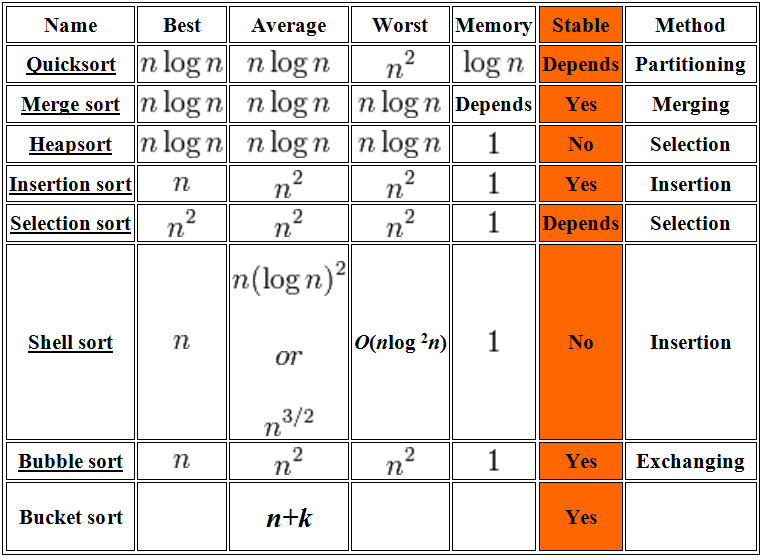
\includegraphics[height=0.65\textheight]{figure/chap07/09stlsort}
  \end{center}
\end{frame}

\begin{frame}[t, fragile]{算法}{修改操作}
  \begin{itemize}
  \item 排序算法
  \end{itemize}
  \begin{center}
    \begin{tikzpicture}[font=\tiny, show background grid]
      \tikzset{coord/.style={coordinate}}
      \umlnote[scale=0.55, text width=0.85\textwidth] (code1) at (0, 0)
      {
        \cppfilenobg{codes/chap07/22-sort2.cpp}
      };
    \end{tikzpicture}
  \end{center}
\end{frame}

\begin{frame}[t, fragile]{算法}{修改操作}
  \begin{itemize}
  \item 堆算法
  \end{itemize}
  \begin{tabbing}
    \cppinline{push_heap} \hspace{4em} \= Push element into heap range\\ 
    \cppinline{pop_heap} \> Pop element from heap range\\ 
    \cppinline{make_heap} \> Make heap from range\\ 
    \cppinline{sort_heap} \> Sort elements of heap 
  \end{tabbing}
  \begin{center}
    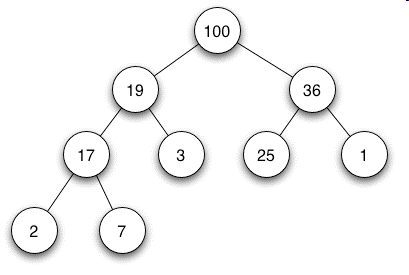
\includegraphics[width=0.45\textwidth]{figure/chap07/10heap}
  \end{center}
\end{frame}

\begin{frame}[t, fragile, ]{算法}{修改操作}
  \begin{itemize}
  \item 堆排序\cppinline{sort_heap}
  \end{itemize}
  \begin{center}
    \begin{tikzpicture}[font=\tiny, show background grid]
      \tikzset{coord/.style={coordinate}}
      \umlnote[scale=0.7, text width=0.85\textwidth] (code1) at (0, 0)
      {
        \cppfilenobg{codes/chap07/23-heap.cpp}
      };
    \end{tikzpicture}
  \end{center}
\end{frame}

\begin{frame}[t, fragile]{算法}{修改操作}
  \begin{itemize}
  \item 二分查找
  \end{itemize}
  \begin{tabbing}
    \cppinline{lower_bound} \hspace{3em} \= Return iterator to lower bound\\ 
    \cppinline{upper_bound} \> Return iterator to upper bound\\ 
    \cppinline{equal_range} \> Get subrange of equal elements\\ 
    \cppinline{binary_search} \> Test if value exists in sorted array     
  \end{tabbing}
  \begin{center}
    \begin{tikzpicture}[font=\tiny, show background grid]
      \tikzset{coord/.style={coordinate}}
      \node[fill=blue!25, draw] (note2) at (0, 0) {\alert{前提}: 操作
        的对象序列已经排序};      
    \end{tikzpicture}
  \end{center}
\end{frame}

\begin{frame}[t, fragile]{算法}{修改操作}
  \begin{itemize}
  \item 二分查找\cppinline{binary_search}
  \end{itemize}
  \begin{center}
    \begin{tikzpicture}[font=\tiny, show background grid]
      \tikzset{coord/.style={coordinate}}
      \umlnote[scale=0.65, text width=0.85\textwidth] (code1) at (0, 0)
      {
        \cppfilenobg{codes/chap07/24-bisearch.cpp}
      };
    \end{tikzpicture}
  \end{center}
\end{frame}

\begin{frame}[t, fragile]{算法}{修改操作}
  \begin{itemize}
  \item 合并
  \end{itemize}  
  \begin{mytabbing}[\scriptsize]    
    \cppinline{merge} \hspace{11em} \= Merge sorted ranges\\
    \cppinline{inplace_merge} \> Merge consecutive sorted ranges\\
    \cppinline{includes} \> Whether sorted range includes another range\\
    \cppinline{set_union} \> Union of two sorted ranges\\
    \cppinline{set_intersection} \> Intersection of two sorted ranges\\
    \cppinline{set_difference} \> Difference of two sorted ranges\\
    \cppinline{set_symmetric_difference} \> Symmetric difference of two sorted ranges
  \end{mytabbing}
  \begin{center}
    \begin{tikzpicture}[font=\tiny, show background grid]
      \tikzset{coord/.style={coordinate}}
      \node[fill=blue!25, draw] (note2) at (0, 0) {\alert{前提}: 操作
        的对象序列已经排序};      
    \end{tikzpicture}
  \end{center}
\end{frame}

\begin{frame}[t, fragile]{算法}{修改操作}
  \begin{itemize}
  \item 求交集\cppinline{set_intersection}
  \end{itemize}
  \begin{center}
    \begin{tikzpicture}[font=\tiny, show background grid]
      \tikzset{coord/.style={coordinate}}
      \umlnote[scale=0.95, text width=0.85\textwidth] (code1) at (0, 0)
      {
        \cppfilenobg{codes/chap07/25-set_intersection.cpp}
      };
    \end{tikzpicture}
  \end{center}
\end{frame}

\begin{frame}[t, fragile]{算法}{修改操作}
  \begin{itemize}
  \item 最小最大值
  \end{itemize}
  \begin{mytabbing}[\scriptsize]
    \cppinline{min} \hspace{12em} \= Return the lesser of two arguments\\
    \cppinline{max} \> Return the greater of two arguments\\
    \cppinline{min_element} \> Return smallest element in range\\
    \cppinline{max_element} \> Return largest element in range\\
    \cppinline{lexicographical_compare} \> Lexicographical less-than comparison\\
    \cppinline{next_permutation} \> Transform range to next permutation\\
    \cppinline{prev_permutation} \> Transform range to previous permutation 
  \end{mytabbing}
\end{frame}

\begin{frame}[t, fragile]{算法}{修改操作}
  \begin{itemize}
  \item 求最大值\cppinline{max_element}
  \end{itemize}
  \begin{center}
    \begin{tikzpicture}[font=\tiny, show background grid]
      \tikzset{coord/.style={coordinate}}
      \umlnote[scale=0.65, text width=0.95\textwidth] (code1) at (0, 0)
      {
        \cppfilenobg{codes/chap07/26-max.cpp}
      };
    \end{tikzpicture}
  \end{center}
\end{frame}

%%%%%%%%%%%%%%%%%%%%%%%%%%%%%%%%%%%%%%%%%%%%%%%%%%%%%%%%%%%%%%%%

\subsection[函数对象]{函数对象}\label{sec:chap07-sec03-05}
%%%%%%%%%%%%%%%%%%%%%%%%%%%%%%%%%%%%%%%%%%%%%%%%%%%%%%%%%%%%%%%%
\begin{frame}[t, fragile]{函数对象}{简介}%
  \begin{itemize}
  \item 函数对象  
  \end{itemize}
  \begin{center}
    \begin{tikzpicture}[font=\tiny, show background grid]
      \tikzset{ coord/.style={coordinate} }
      \node[text width=0.85\textwidth] (fig1) at (0, 0)
      {
        \centering
        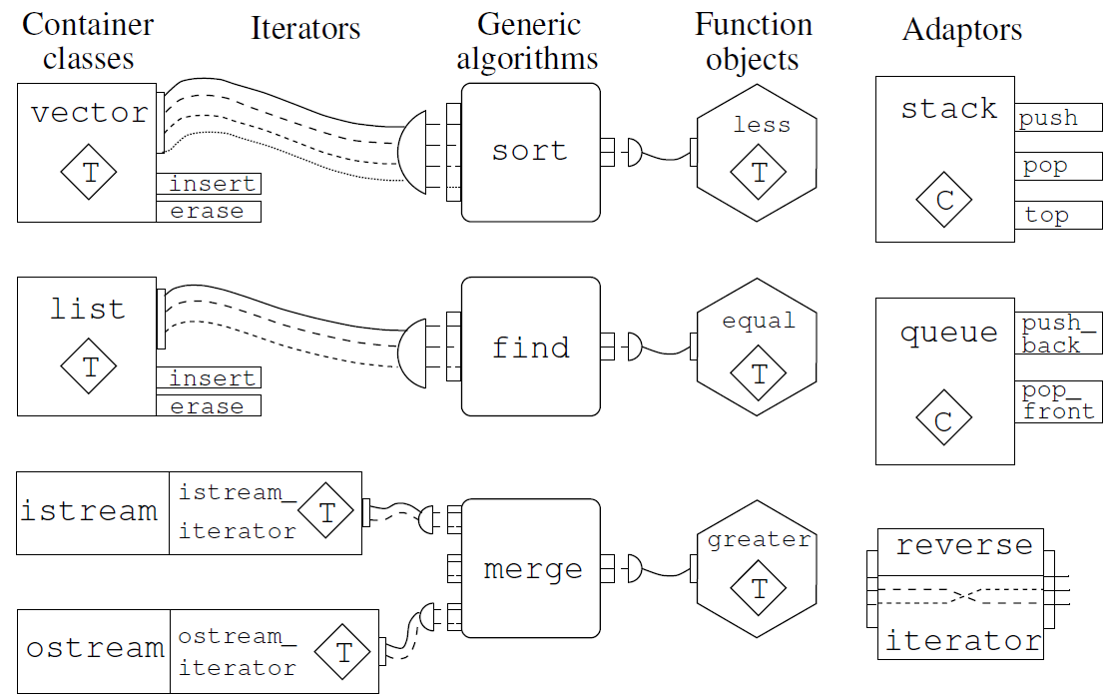
\includegraphics[width=0.95\textwidth]{figure/chap07/02stl04}
      };

      \path let \p1=(fig1) in
      coordinate (org) at (\x1, \y1)
      coordinate (ovBL1) at ($(org) + (0.9, -2.85)$)
      coordinate (ovUR1) at ($(ovBL1) + (1.40, 6.1)$)
      ;

      \draw[fill=green!25, red, thick, opacity=0.3] (ovBL1) rectangle (ovUR1);
    \end{tikzpicture}
  \end{center}  
\end{frame}

% \begin{frame}[t, fragile]{函数对象}%
%   \begin{itemize}
%   \item 定义
%   \item 与普通函数区别
%   \item 系统预定义的函数对象
%   \end{itemize}
% \end{frame}

\begin{frame}[t, fragile]{函数对象}{函数对象定义}%
  \begin{itemize}
  \item 定义
    \begin{itemize}
    \item 函数调用运算符()
    \item 如果某个类重载了(),该类的实例就是一个函数对象
    \end{itemize}
    \begin{center}
      \begin{minipage}[t]{0.65\linewidth}
        \begin{cppttnobg}
struct MyClass
{
  |返回值| operator()(|参数列表|) {}
};

MyClass myObj;
myObj(|实参|);
        \end{cppttnobg}
      \end{minipage}
    \end{center}
  \item 优点
    \begin{itemize}
    \item 使用灵活,可包含状态信息
    \item 可当作数据类型作为模板参数传递
    \end{itemize}
  \end{itemize}
\end{frame}

\begin{frame}[t, fragile]{函数对象}{与普通函数区别}
  \begin{itemize}
  \item 例1
  \end{itemize}
  \begin{center}
    \begin{tikzpicture}[font=\tiny, show background grid]
      \tikzset{coord/.style={coordinate}}
      \umlnote[scale=0.95, text width=0.45\textwidth] (code1) at (0, 0)
      {
        \cppfilenobg{codes/chap07/27-funobj.cpp}
      };
    \end{tikzpicture}
  \end{center}
\end{frame}

\begin{frame}[t, fragile]{函数对象}{与普通函数区别}
  \begin{itemize}
  \item 例1
  \end{itemize}
  \begin{center}
    \begin{tikzpicture}[font=\tiny, show background grid]
      \tikzset{coord/.style={coordinate}}
      \umlnote[scale=1.0, text width=0.5\textwidth] (code1) at (0, 0)
      {
        \cppfilenobg{codes/chap07/27-funobjmain01.cpp}
      };
    \end{tikzpicture}
  \end{center}
\end{frame}

\begin{frame}[t, fragile]{函数对象}{与普通函数区别}
  \begin{itemize}
  \item 例2
  \end{itemize}
  \begin{center}
    \begin{tikzpicture}[font=\tiny, show background grid]
      \tikzset{coord/.style={coordinate}}
      \umlnote[scale=1.0, text width=0.5\textwidth] (code1) at (0, 0)
      {
        \cppfilenobg{codes/chap07/27-funobjmain02.cpp}
      };
    \end{tikzpicture}
  \end{center}
\end{frame}

\begin{frame}[t, fragile]{函数对象}{与普通函数区别}
  \begin{itemize}
  \item 例2
  \end{itemize}
  \begin{center}
    \begin{tikzpicture}[font=\tiny, show background grid]
      \tikzset{coord/.style={coordinate}}
      \umlnote[scale=0.65, text width=0.45\textwidth] (code1) at (0, 0)
      {
        \cppfilenobg{codes/chap07/28-funobj.cpp}
      };
    \end{tikzpicture}
  \end{center}
\end{frame}

\begin{frame}[t, fragile]{函数对象}{与普通函数区别}
  \begin{itemize}
  \item 例2
  \end{itemize}
  \begin{center}
    \begin{tikzpicture}[font=\tiny, show background grid]
      \tikzset{coord/.style={coordinate}}
      \umlnote[scale=1.0, text width=0.5\textwidth] (code1) at (0, 0)
      {
        \cppfilenobg{codes/chap07/28-funobjmain01.cpp}
      };
    \end{tikzpicture}
  \end{center}
\end{frame}

\begin{frame}[t, fragile]{函数对象}{系统预定义函数对象}%
  \begin{itemize}
  \item 算术操作Arithmetic operations
  \item 比较操作Comparison operations
  \item 逻辑操作Logical operations
  \item 其它
  \end{itemize}
\end{frame}

\begin{frame}[t, fragile]{函数对象}{系统预定义函数对象}
  \begin{itemize}
  \item 算术操作
  \end{itemize}
  \begin{tabbing}
    \cppinline{plus} \hspace{3em} \= Addition function object class\\ 
    \cppinline{minus} \> Subtraction function object class\\
    \cppinline{multiplies} \> Multiplication function object class\\
    \cppinline{divides} \> Division function object class\\
    \cppinline{modulus} \> Modulus function object class\\
    \cppinline{negate} \> Negative function object class 
  \end{tabbing}
\end{frame}

\begin{frame}[t, fragile]{函数对象}{系统预定义函数对象}%
  \begin{itemize}
  \item 算术操作    
  \end{itemize}
  \begin{center}
    \begin{minipage}[t]{0.65\linewidth}
      \begin{cppttnobg}
template <class T>
struct plus : binary_function <T,T,T>
{
  T operator() (const T& x, const T& y) const
  {
    return x+y;
  }
};
      \end{cppttnobg}
    \end{minipage}
  \end{center}
\end{frame}

\begin{frame}[t, fragile]{函数对象}{算术操作}
  \begin{itemize}
  \item plus类模板
  \end{itemize}
  \begin{center}
    \begin{tikzpicture}[font=\tiny, show background grid]
      \tikzset{coord/.style={coordinate}}
      \umlnote[scale=1.15, text width=0.605\textwidth] (code1) at (0, 0)
      {
        \cppfilenobg{codes/chap07/29-funobjplus.cpp}
      };

      \path let \p1=(code1) in
      coordinate (org) at (\x1, \y1)
      coordinate (ovBL1) at ($(org) + (-4.6, 1.73)$)
      coordinate (ovUR1) at ($(ovBL1) + (2.75, 0.26)$)
      ;

      \path let \p1=(code1) in
      coordinate (org) at (\x1, \y1)
      coordinate (ovBL2) at ($(org) + (1.00, -1.00)$)
      coordinate (ovUR2) at ($(ovBL2) + (1.58, 0.33)$)
      ;

      \draw[fill=green!25, red, thick, fill opacity=0.3] (ovBL1) rectangle
      (ovUR1);

      \draw[fill=green!25, red, thick, fill opacity=0.3] (ovBL2) rectangle
      (ovUR2);
      
    \end{tikzpicture}
  \end{center}
\end{frame}


\begin{frame}[t, fragile]{函数对象}{系统预定义函数对象}
  \begin{itemize}
  \item 比较操作
  \end{itemize}
  \begin{tabbing}
    \cppinline{equal_to} \hspace{3em} \= Function object class for
    equality\\ \> comparison\\
    \cppinline{not_equal_to} \> Non-equality comparison\\
    \cppinline{greater} \> Greater-than inequality comparison\\
    \cppinline{less} \> Less-than inequality comparison\\
    \cppinline{greater_equal} \> Greater-than-or-equal-to comparison\\
    \cppinline{less_equal} \> Less-than-or-equal-to comparison 
  \end{tabbing}
\end{frame}

\begin{frame}[t, fragile]{函数对象}{比较操作}
  \begin{itemize}
  \item 大于操作greater
  \end{itemize}
  \begin{center}
    \begin{tikzpicture}[font=\tiny, show background grid]
      \tikzset{coord/.style={coordinate}}
      \umlnote[scale=1.3, text width=0.53\textwidth] (code1) at (0, 0)
      {
        \cppfilenobg{codes/chap07/30-funobjgreater.cpp}
      };

      \path let \p1=(code1) in
      coordinate (org) at (\x1, \y1)
      coordinate (ovBL1) at ($(org) + (-0.58, -1.09)$)
      coordinate (ovUR1) at ($(ovBL1) + (2.05, 0.35)$)
      ;

      \draw[fill=green!25, red, thick, fill opacity=0.3] (ovBL1) rectangle
      (ovUR1);      
    \end{tikzpicture}
  \end{center}
\end{frame}

\begin{frame}[t, fragile]{函数对象}{系统预定义函数对象}
  \begin{itemize}
  \item 逻辑操作
  \end{itemize}
  \begin{tabbing}
    \cppinline{logical_and} \hspace{3em} \= Logical AND function object class\\
    \cppinline{logical_or} \> Logical OR function object class\\
    \cppinline{logical_not} \> Logical NOT function object class
  \end{tabbing}
\end{frame}

\begin{frame}[t, fragile]{函数对象}{逻辑操作}%
  \begin{itemize}
  \item 逻辑非操作\cppinline{logical_not}
  \end{itemize}
  \begin{center}
    \begin{minipage}[t]{0.45\linewidth}
      \begin{cppttnobg}
template <class T>
struct logical_not : unary_function <T,bool>
{
  bool operator() (const T& x) const
  {
    return !x;
  }
};
      \end{cppttnobg}
    \end{minipage}
  \end{center}
\end{frame}

\begin{frame}[t, fragile]{函数对象}{逻辑操作}
  \begin{itemize}
  \item 逻辑非操作\cppinline{logical_not}
  \end{itemize}
  \begin{center}
    \begin{tikzpicture}[font=\tiny, show background grid]
      \tikzset{coord/.style={coordinate}}
      \umlnote[scale=1.2, text width=0.6\textwidth] (code1) at (0, 0)
      {
        \cppfilenobg{codes/chap07/31-funobjlogicalnot.cpp}
      };

      \path let \p1=(code1) in
      coordinate (org) at (\x1, \y1)
      coordinate (ovBL1) at ($(org) + (0.25, -0.71)$)
      coordinate (ovUR1) at ($(ovBL1) + (2.6, 0.32)$)
      ;

      \draw[fill=green!25, red, thick, fill opacity=0.3] (ovBL1) rectangle
      (ovUR1);      
    \end{tikzpicture}
  \end{center}
\end{frame}
%%%%%%%%%%%%%%%%%%%%%%%%%%%%%%%%%%%%%%%%%%%%%%%%%%%%%%%%%%%%%%%%

\section[第3方库]{第3方库}\label{sec:chap07-sec04}
%%%%%%%%%%%%%%%%%%%%%%%%%%%%%% 继承的方式 %%%%%%%%%%%%%%%%%%%%%%%%%%%%%%%%%%
\begin{frame}[t, fragile]{第3方库}{STL未涉及内容}%
  \begin{itemize}
  \item 树
  \item 图
  \item 其它
    \begin{itemize}
    \item 矩阵运算
    \item 正则表达式
    \item 智能指针
    \item 高斯分布随机数
    \item 多线程操作等
    \end{itemize}
  \end{itemize}
\end{frame}

\begin{frame}[t, fragile]{第3方库}{树的表示}%
  \begin{itemize}
  \item Core::tree(适合在VS下编译)\\
    {\tiny \url{http://archive.gamedev.net/archive/reference/programming/features/coretree2/page5.html}}
  \item Tree.hh: an STL-like C++ tree class\\
    {\tiny \url{http://tree.phi-sci.com/documentation.html}}
  \end{itemize}
  \begin{center}
    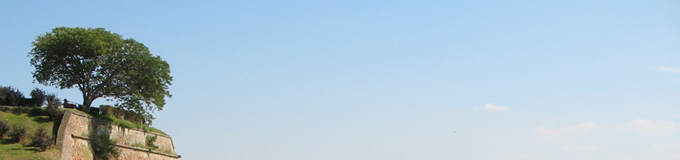
\includegraphics[width=0.8\textwidth]{figure/chap07/11tree}
  \end{center}
\end{frame}

\begin{frame}[t, fragile]{第3方库}{Boost}%
  \begin{itemize}
  \item 一组扩充C++功能性的经过同行评审(Peer-reviewed)且开放源代码程序库。
  \item 开源代码。{ \url{http://www.boost.org/}}
  \item 许多Boost的开发人员来自C++标准委员会,而部份的Boost库成为C++的TR1标准之一。
  \end{itemize}
  \begin{center}
    
\includegraphics[width=0.4\textwidth]{figure/chap07/12boost}\\
    {\tiny \url{http://mail.ustc.edu.cn/~jxw95216/boost_doc/libs/libraries.htm}}
    {\tiny \url{http://www.kmonos.net/alang/boost/}}
  \end{center}  
\end{frame}

\begin{frame}[t, fragile]{第3方库}{Boost}%
  \begin{itemize}
  \item 分类库列表
    \begin{itemize}
      \scriptsize
    \item String and text processing 字符串与文本处理
    \item Containers 容器
    \item Iterators 迭代器
    \item Algorithms 算法
    \item Function Objects and higher-order programming 函数对象与高阶
      编程
    \item Generic Programming 泛型编程
    \item Template Metaprogramming 模板元编程
    \item Preprocessor Metaprogramming 预处理元编程
    \item Concurrent Programming 并发编程
    \item Math and numerics 数学与数字
    \item Correctness and testing 正确性与测试
    \item Data structures 数据结构
    \item Image processing 图像处理
    \item Input/Output 输入/输出
    \item Inter-language support 交叉语言支持
    \item Memory 内存
    \item Parsing 语法分析
    \item Programming Interfaces 编程接口
    \item Miscellaneous 杂项
    \item Broken compiler workarounds 不合标准的编译器支持
    \end{itemize}
  \end{itemize}
\end{frame}

\begin{frame}[t, fragile]{第3方库}{Boost}%
  \begin{itemize}
  \item 安装与编译
    \begin{itemize}
    \item \cppinline{date_time, regex, thread, python, signals, test, filesystem, serialization, program_options} 需要bjam进行编译生成*.lib文件;\\
        VS: {\url{http://www.boostpro.com/download/}}
      \item 其余组件只需包含相应头文件即可。
    \end{itemize}
  \end{itemize}
  \begin{center}
    
\includegraphics[width=0.45\textwidth]{figure/chap07/12boost}
  \end{center}
\end{frame}

%%%%%%%%%%%%%%%%%%%%%%%%%%%%%%%%%%%%%%%%%%%%%%%%%%%%%%%%%%%%%%%%%%%%%%%%%%%%%%%
% 附件页
\section[附件下载]{本讲示例代码及附件下载} 
\begin{frame}{附件}{本讲附件}
  % 此处的[ucfilespec=...]必须指定为pdf否则Windows下无法下载
  %\vspace{-4ex}
  \textattachfile[ucfilespec=ex-src07.pdf]{ex-src07.zip}{附件:右键单击该
    链接,选择\qtmark{\alert{保存附件}}下载,\alert{将后缀名改为\qtmark{.zip}解压}
      \footnote[frame]{请\alert{退出全屏模式}后点击该链接。}
      \footnote[frame]{以Adobe Acrobat Reader为例。}
      。}%\\

  \vspace{-1ex}
  \begin{center}
    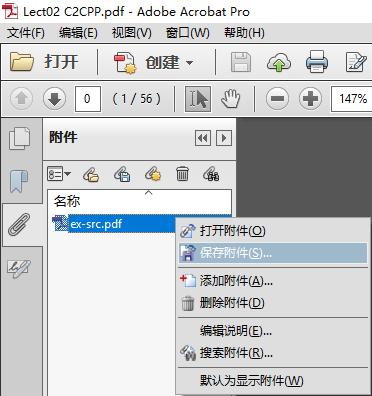
\includegraphics[height=0.35\textheight]{pdfattatchdownload01}\quad
    %或 \quad%
    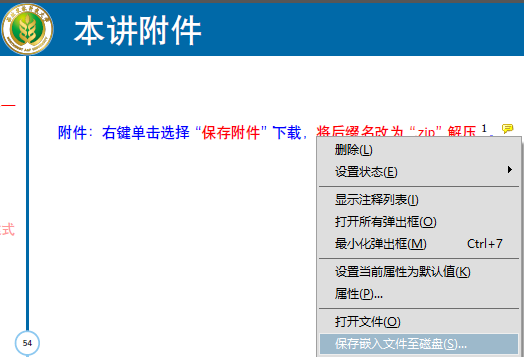
\includegraphics[height=0.35\textheight]{pdfattatchdownload02}\\[2ex]%
    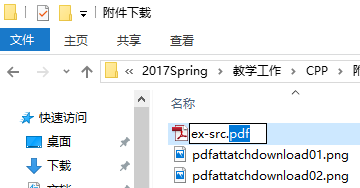
\includegraphics[height=0.255\textheight]{pdfattatchdownload03}\quad
    %$\Rightarrow$ \quad%
    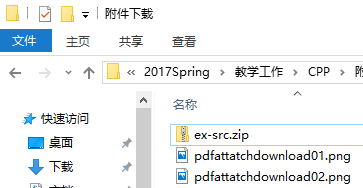
\includegraphics[height=0.255\textheight]{pdfattatchdownload04}%
  \end{center}   
\end{frame}

% \tiny
% \scriptsize
% \footnotesize
% \small
% \normalsize
% \large
% \Large
% \LARGE
% \huge
% \Huge


%%% Local Variables: 
%%% mode: latex
%%% TeX-master: "../main.tex"
%%% End: 
